\documentclass[12pt, a4paper]{article}

% ==========================================
% 1. KHAI BÁO GÓI THƯ VIỆN (PACKAGES)
% ==========================================
% Bảng mã & Font chữ
\usepackage[utf8]{inputenc}
\usepackage[T5]{fontenc}

% Toán học
\usepackage{amsmath, amssymb}

% Căn lề & Bố cục trang
\usepackage[top=2.2cm, bottom=1.5cm, left=1cm, right=1cm, headheight=15pt]{geometry}
\usepackage{fancyhdr}
\usepackage{needspace}
\usepackage{tkz-tab}
\usepackage{float}

% Đồ họa & Màu sắc
\usepackage{xcolor}
\usepackage{graphicx} 
\usepackage{tikz}
\usetikzlibrary{calc, shapes.geometric, positioning}


% Bảng biểu & Danh sách
\usepackage{colortbl}
\usepackage{array}
\usepackage{makecell}
\usepackage{multirow}
\usepackage{tasks}

% Biểu tượng
\usepackage{fontawesome5}

% ==========================================
% 2. THIẾT LẬP MÀU SẮC CHỦ ĐẠO
% ==========================================
\definecolor{goldyellow}{RGB}{255, 179, 0}
\definecolor{amberorange}{RGB}{230, 115, 0}
\definecolor{lightamber}{RGB}{255, 248, 225}
\definecolor{deepblue}{RGB}{25, 42, 86}
\definecolor{accentred}{RGB}{232, 65, 24}
\definecolor{softgray}{RGB}{220, 220, 222} 
\definecolor{fbblue}{RGB}{15, 80, 200}


% ==========================================
% 3. CẤU HÌNH HEADER & FOOTER
% ==========================================
\pagestyle{fancy}
\fancyhf{}
\renewcommand{\headrulewidth}{0pt}

% Khai báo biến lưu trữ nội dung góc phải của Header
\newcommand{\HeaderRightText}{}

% --- Header ---
\fancyhead[C]{
    \begin{tikzpicture}[remember picture, overlay]
        
        % Dải màu trang trí góc trên
        \path[fill=deepblue] (current page.north west) -- (current page.north east) 
            -- ($(current page.north east) + (0, -1.6cm)$) 
            .. controls ($(current page.north) + (3, -2.0cm)$) and ($(current page.north) + (-3, -0.4cm)$) .. 
            ($(current page.north west) + (0, -1.0cm)$) -- cycle;
            
        \path[fill=goldyellow] (current page.north west) -- (current page.north east) 
            -- ($(current page.north east) + (0, -1.0cm)$) 
            .. controls ($(current page.north) + (4, -1.0cm)$) and ($(current page.north) + (-2, -2.2cm)$) .. 
            ($(current page.north west) + (0, -1.6cm)$) -- cycle;
            
        \path[fill=amberorange] (current page.north west) -- ($(current page.north west) + (6.5cm, 0)$) 
            .. controls ($(current page.north west) + (4.5cm, -1.2cm)$) and ($(current page.north west) + (2cm, -2.0cm)$) .. 
            ($(current page.north west) + (0, -2.0cm)$) -- cycle;
            
        % Logo góc trái Header
        \node[anchor=west, inner sep=0pt] 
            at ($(current page.north west) + (0cm, -0.8cm)$) {
\includegraphics[height=2.0cm]{../../../image/logo-header.png}};
            
        % Text góc phải Header (Tự động lấy từ đối số thứ 3 của \titlebox)
        \node[anchor=east, text=white, font=\small\bfseries\sffamily] 
            at ($(current page.north east) + (-0.8cm, -0.5cm)$) {\HeaderRightText};
    \end{tikzpicture}
}

% --- Footer ---
\fancyfoot[C]{
    \begin{tikzpicture}[remember picture, overlay]
        % Đường kẻ ngang
        \draw[amberorange, line width=1.5pt] 
            ($(current page.south west) + (0cm, 0.4cm)$) -- ($(current page.south east) + (0cm, 0.4cm)$);

        % Dải cong góc phải
        \path[fill=goldyellow] (current page.south east) -- ($(current page.south east) + (-5cm, 0)$) 
            .. controls ($(current page.south east) + (-3cm, 0.8cm)$) and ($(current page.south east) + (-1.5cm, 1.2cm)$) .. 
            ($(current page.south east) + (0, 1.2cm)$) -- cycle;

        % Mạng xã hội
        \node[anchor=west, inner sep=0pt] at ($(current page.south west) + (1cm, 0.8cm)$) {
            \small\sffamily
            \textcolor{fbblue}{\faFacebook\hskip 4pt Toán Anh Huy MATH-STER}
            \hskip 18pt
            \textcolor{black}{\faTiktok\hskip 4pt huymathster}
        };

        % Số trang
        \node[circle, fill=white, draw=amberorange, line width=1.5pt, text=deepblue, font=\large\bfseries\sffamily, inner sep=4pt, minimum size=0.8cm] 
            at ($(current page.south east) + (-1.2cm, 0.6cm)$) {\thepage};
    \end{tikzpicture}
}

% ==========================================
% 4. ĐỊNH NGHĨA MACRO: KHUNG TIÊU ĐỀ
% ==========================================
\newcommand{\titlebox}[3]{
    % Gán nội dung đối số #3 vào biến HeaderRightText
    \gdef\HeaderRightText{#3}
    
    \begin{center}
    \vspace*{-0.5cm}
    \begin{tikzpicture}
        % Khung vô hình (Phantom Box) định chuẩn kích thước
        \node[text width=16cm, inner xsep=0pt, inner ysep=16pt, opacity=0] (MainBox) {
            \begin{minipage}[c]{4.2cm}
                \centering\vspace{0.1cm}
                \rule{2.2cm}{2.2cm} 
                \vspace{0.1cm}
            \end{minipage}%
            \begin{minipage}[c]{11.5cm}
                \centering\vspace{0.15cm}
                {\huge\bfseries\sffamily #2 \par}
                \vspace{0.15cm} 
            \end{minipage}
        };
        
        % Đổ bóng & Nền
        \fill[goldyellow, rounded corners=8pt] ([xshift=5pt, yshift=-5pt]MainBox.south west) rectangle ([xshift=5pt, yshift=-5pt]MainBox.north east);
        \fill[white, rounded corners=8pt] (MainBox.south west) rectangle (MainBox.north east);
        
        % Lưới ô ly & Nền Logo
        \begin{scope}
            \clip[rounded corners=8pt] (MainBox.south west) rectangle (MainBox.north east);
            \draw[step=0.4cm, softgray!50, line width=0.6pt] (MainBox.south west) grid (MainBox.north east);
            \fill[lightamber!60] (MainBox.south west) rectangle ([xshift=4.2cm]MainBox.north west);
        \end{scope}

        % Viền ngoài
        \draw[deepblue, line width=1.5pt, rounded corners=8pt] (MainBox.south west) rectangle (MainBox.north east);

        % Nội dung Text (Lớp trên cùng)
        \node[text width=16cm, inner xsep=0pt, inner ysep=16pt] at (MainBox.center) {
            \begin{minipage}[c]{4.2cm}
                \centering
                % --- ĐIỀU CHỈNH TỌA ĐỘ LOGO Ở ĐÂY ---
                \hspace*{-0.5cm}\raisebox{-0.2cm}{
\includegraphics[width=5.5cm]{../../../image/logo.png}}
            \end{minipage}%
            \begin{minipage}[c]{11.5cm}
                \centering\vspace{0.15cm}
                {\huge\bfseries\sffamily\color{deepblue} #2 \par}
                \vspace{0.15cm} 
            \end{minipage}
        };
        
        % Trang trí phụ kiện
        \draw[deepblue, line width=1.5pt, dashed] ([xshift=4.2cm]MainBox.north west) -- ([xshift=4.2cm]MainBox.south west);
        \node[regular polygon, regular polygon sides=4, rotate=45, fill=white, draw=accentred, line width=1.2pt, inner sep=2.5pt] at ([xshift=4.2cm]MainBox.west) {};
        \node[anchor=west, fill=amberorange, text=white, font=\large\bfseries\sffamily, rounded corners=4pt, draw=deepblue, line width=1.5pt, inner xsep=12pt, inner ysep=6pt] at ([xshift=1.5cm]MainBox.north west) {#1};
        \fill[accentred] ([xshift=-1.8cm, yshift=-0.4cm]MainBox.north east) circle (3pt);
        \fill[amberorange] ([xshift=-1.4cm, yshift=-0.4cm]MainBox.north east) circle (3pt);
        \fill[goldyellow] ([xshift=-1.0cm, yshift=-0.4cm]MainBox.north east) circle (3pt);
    \end{tikzpicture}
    \vspace*{0cm}
    \end{center}
}

% ==========================================
% 5. ĐỊNH NGHĨA MACRO: CẤU TRÚC CÂU HỎI (ÉP SÁT NHAU)
% ==========================================
\newcommand{\questioncore}[2]{
    % Xóa khoảng cách phía trên, ép sát câu trước
    \noindent \textbf{\textcolor{deepblue}{Câu #1.} \textcolor{accentred}{[STER]}} #2
    \par\nopagebreak
}

% Cấu hình hiển thị đáp án trắc nghiệm
\settasks{
    label=\textbf{\textcolor{amberorange}{\Alph*.}}, 
    label-width=15pt,     
    item-indent=25pt,     
    label-offset=6pt,    
    column-sep=20pt,     
    after-item-skip=2pt  % Đã giảm tối đa khoảng cách giữa các dòng đáp án A B C D
}

% Hàm vẽ dòng kẻ nháp
\newcommand{\drawdashlines}[1]{
    \ifnum#1>0
        \nopagebreak\vspace{0.1cm}\noindent 
        \begin{tikzpicture}
            \foreach \i in {1,...,#1} {
                \draw[softgray, line width=0.2pt] (0,-{\i*0.75}) -- (\textwidth-4pt,-{\i*0.75});
            }
        \end{tikzpicture}
        \par
    \fi
    % Đã xóa hoàn toàn khoảng cách thừa ở nhánh else
}

% --- Dạng 1: Trắc nghiệm 4 đáp án ---
\newcommand{\questionLinesManual}[4]{
    \pgfmathsetmacro{\calculatedSpace}{1.5 + #1 * 0.65}
    \needspace{\calculatedSpace cm} 
    \questioncore{#2}{#3}
    #4
    \par\nopagebreak
    \drawdashlines{#1}
}

% --- Dạng 2: Trắc nghiệm Đúng/Sai ---
\newcommand{\questionTrueFalse}[4]{
    \pgfmathsetmacro{\calculatedSpace}{3.0 + #1 * 0.65} 
    \needspace{\calculatedSpace cm}
    \questioncore{#2}{#3}
    
    \nopagebreak
    \begin{center}
    \renewcommand{\arraystretch}{1.8} % Bóp nhỏ chiều cao của bảng Đ/S
    \begin{tabular}{|>{\centering\arraybackslash}m{0.8cm}|m{12cm}|>{\centering\arraybackslash}m{2cm}|>{\centering\arraybackslash}m{2cm}|}
        \hline
        \rowcolor{amberorange!20}
        & \multicolumn{1}{>{\centering\arraybackslash}m{12cm}|}{\textbf{\textcolor{deepblue}{Mệnh đề}}} & 
        \textbf{\textcolor{deepblue}{Đúng}} & 
        \textbf{\textcolor{deepblue}{Sai}} \\
        \hline
        #4
        \hline
    \end{tabular}
    \renewcommand{\arraystretch}{1}
    \end{center}
    
    \par\nopagebreak
    \drawdashlines{#1}
}

% ----- Dạng 3: Tự luận ngắn -----
\newcommand{\questionShortAnswer}[3]{
    \pgfmathsetmacro{\calculatedSpace}{1.5 + #1 * 0.8}
    \needspace{\calculatedSpace cm}
    
    {\linespread{1.1}\selectfont % Bóp nhỏ giãn dòng của câu tự luận
    \questioncore{#2}{#3}\par}
    
    \nopagebreak
    \begin{flushright}
        \begin{tikzpicture}
            \node[anchor=east, font=\small\bfseries\sffamily, text=deepblue] 
                at (-0.2, 0.4) {Đáp án:};
            \fill[goldyellow, rounded corners=3pt] (0.08, -0.08) rectangle (3.08, 0.72);
            \draw[draw=deepblue, fill=white, line width=1.2pt, rounded corners=3pt] 
                (0,0) rectangle (3.0, 0.8);
            \foreach \x in {0.75, 1.5, 2.25} {
                \draw[draw=deepblue, line width=0.6pt] (\x, 0) -- (\x, 0.8);
            }
        \end{tikzpicture}
    \end{flushright}
    
    \par\nopagebreak
    \drawdashlines{#1}
}

% ==========================================
% BẮT ĐẦU NỘI DUNG TÀI LIỆU
% ==========================================
\begin{document}

% Truyền 3 tham số: {Nhãn cam} {Chữ to chính giữa} {Chữ ở góc phải Header}
\titlebox{Chủ đề: Hàm số}{Giá trị lớn nhất nhỏ nhất của quảng đường}{Hàm số: Min Max quảng đường}

% --- CÂU 1 ---
\questionTrueFalse{0}{1}{Một kho hàng được đặt tại vị trí A cách trục đường chính một khoảng \( AB = 8 \, km \). Trên trục đường đó có một trung tâm thương mại ở vị trí C cách B một khoảng \( BC = 20 \, km \) (tham khảo hình vẽ). Người giao hàng có thể đi xe máy từ vị trí A đến vị trí M trên trục đường chính với vận tốc 40 km/h và đi xe ô tô đến trung tâm thương mại C với vận tốc 60 km/h. Đặt \( BM = x \) với \( 0 < x < 20 \).
\begin{center}
    \begin{tikzpicture}[>=stealth, scale=1.3]

    % =================================================================
    % 1. ĐỊNH NGHĨA CÁC ĐIỂM CHÍNH TRÊN TRỤC HOÀNH VÀ ĐƯỜNG CAO
    % =================================================================
    % Trục nằm ngang kéo dài sang hai bên một chút
    \coordinate (StartLine) at (-0.5,0);
    \coordinate (EndLine) at (5.0,0);
    
    % Các điểm chính
    \coordinate (B) at (0.3,0);
    \coordinate (M) at (2.2,0);
    \coordinate (C) at (4.5,0);
    \coordinate (A) at (0.3,3.0);

    % =================================================================
    % 2. VẼ CÁC ĐƯỜNG THẲNG
    % =================================================================
    % Vẽ đường thẳng nằm ngang chính
    \draw[thick] (StartLine) -- (EndLine);

    % Vẽ đoạn thẳng đứng AB và đoạn thẳng nghiêng AM
    \draw[thick] (A) -- (B);
    \draw[thick] (A) -- (M);

    % =================================================================
    % 3. VẼ KÝ HIỆU GÓC VUÔNG VÀ ĐIỂM ĐẶC BIỆT
    % =================================================================
    % Ký hiệu góc vuông tại đỉnh B (nằm bên trái đoạn thẳng AB)
    \draw[thin] (B) ++(-0.18,0) -- ++(0,0.18) -- ++(0.18,0);

    % Điểm C được biểu diễn bằng một chấm tròn đen nhỏ
    \fill (C) circle (1.5pt);

    % =================================================================
    % 4. GÁN NHÃN CÁC ĐỈNH
    % =================================================================
    \node[left=3pt] at (A) {$A$};
    \node[below=3pt] at (B) {$B$};
    \node[below=3pt] at (M) {$M$};
    \node[below=3pt] at (C) {$C$};

\end{tikzpicture}
\end{center}
}{
    \textbf{a)} & Quãng đường đi từ A đến M là \( 64 + x^2 \, (km) \).
    & \textcolor{amberorange}{$\bigcirc$} & \textcolor{amberorange}{$\bigcirc$} \\ \hline
    
    \textbf{b)} & Thời gian đi từ A đến C là \( 40\sqrt{64 + x^2} + 60(20 - x) \) giờ.
    & \textcolor{amberorange}{$\bigcirc$} & \textcolor{amberorange}{$\bigcirc$} \\ \hline
    
    \textbf{c)} & Thời gian ngắn nhất đi từ A đến C là khoảng 29 phút.
    & \textcolor{amberorange}{$\bigcirc$} & \textcolor{amberorange}{$\bigcirc$} \\ \hline
    
    \textbf{d)} & Muộn nhất 7 giờ 1 phút người đó phải xuất phát từ vị trí A để có mặt tại C lúc 8h sáng.
    & \textcolor{amberorange}{$\bigcirc$} & \textcolor{amberorange}{$\bigcirc$} \\
}

% --- CÂU 2 ---
\questionTrueFalse{0}{2}{Trong một cuộc thi cắm trại, xóm Kim Nghĩa treo bóng nháy cho công trại, sao cho điểm đầu và điểm cuối của dây bóng nằm ở vị trí hai chân của cổng. Ban cán sự xóm muốn treo bóng sao cho nó tạo thành hình tam giác như hình vẽ, biết xà ngang chứa điểm C treo bóng cách mặt đất 15m và cổng trại AB rộng 50m. Đặt \( AM = x \) (\( 0 < x < 50 \)) (m).
\begin{center}
    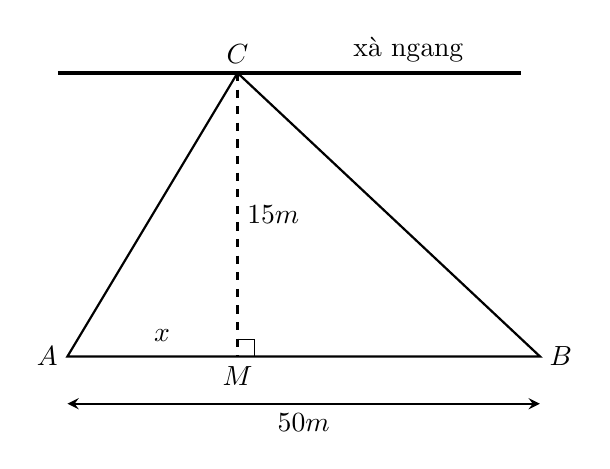
\begin{tikzpicture}[>=stealth, scale=1.2]

    % =================================================================
    % 1. ĐỊNH NGHĨA CÁC ĐIỂM CHÍNH TRONG TAM GIÁC
    % =================================================================
    \coordinate (A) at (0,0);
    \coordinate (B) at (5.0,0);
    \coordinate (M) at (1.8,0);
    \coordinate (C) at (1.8,3.0);

    % Tọa độ hai đầu của thanh xà ngang đi qua C
    \coordinate (XaTrai) at (-0.1,3.0);
    \coordinate (XaPhai) at (4.8,3.0);

    % =================================================================
    % 2. VẼ CÁC ĐƯỜNG LIỀN VÀ XÀ NGANG
    % =================================================================
    % Vẽ thanh xà ngang phía trên bằng nét siêu đậm
    \draw[ultra thick] (XaTrai) -- (XaPhai) node[above left, pos=0.9] {xà ngang};

    % Vẽ các cạnh của tam giác ABC
    \draw[thick] (A) -- (B) -- (C) -- cycle;

    % =================================================================
    % 3. VẼ ĐƯỜNG CAO CM (NẾT ĐỨT) VÀ GÓC VUÔNG
    % =================================================================
    \draw[dashed, thick] (C) -- (M);

    % Ký hiệu góc vuông tại M (nằm bên phải đường cao CM)
    \draw[thin] (M) ++(0,0.18) -- ++(0.18,0) -- ++(0,-0.18);

    % =================================================================
    % 4. GÁN NHÃN CÁC ĐỈNH VÀ THÔNG SỐ TRONG HÌNH
    % =================================================================
    \node[left] at (A) {$A$};
    \node[right] at (B) {$B$};
    \node[below] at (M) {$M$};
    \node[above] at (C) {$C$};

    % Điền giá trị độ dài x và 15m
    \node[above] at (1.0,0.05) {$x$};
    \node[right] at (1.8,1.5) {$15m$};

    % =================================================================
    % 5. VẼ MŨI TÊN KÍCH THƯỚC CHIỀU DÀI 50m PHÍA DƯỚI
    % =================================================================
    \draw[<->, thick] (0,-0.5) -- (5.0,-0.5);
    \node[below] at (2.5,-0.5) {$50m$};

\end{tikzpicture}
\end{center}
}{
    \textbf{a)} & Độ dài đoạn \( CB \) bằng \( \sqrt{15^2 + (50 - x)^2} \) (m).
    & \textcolor{amberorange}{$\bigcirc$} & \textcolor{amberorange}{$\bigcirc$} \\ \hline
    
    \textbf{b)} & Tổng đường dây bóng nối từ \( C \) đến \( A \) và từ \( C \) đến \( B \) là \( \sqrt{x^2 + 15} + \sqrt{(50 - x)^2 + 15} \) (m).
    & \textcolor{amberorange}{$\bigcirc$} & \textcolor{amberorange}{$\bigcirc$} \\ \hline
    
    \textbf{c)} & Khi \( x = 25 \) (m) thì tổng đường dây bóng cần nối là ngắn nhất.
    & \textcolor{amberorange}{$\bigcirc$} & \textcolor{amberorange}{$\bigcirc$} \\ \hline
    
    \textbf{d)} & Biết chi phí mỗi mét dây bóng có giá 15 000 đồng. Chi phí thấp nhất mà ban cán sự xóm cần trả là 874 643 đồng (kết quả làm tròn đến hàng đơn vị).
    & \textcolor{amberorange}{$\bigcirc$} & \textcolor{amberorange}{$\bigcirc$} \\
}

% --- CÂU 3 ---
\questionTrueFalse{0}{3}{Hai vận động viên đang ở vị trí A trên bờ cát, cách bờ biển là 5 km. Hai vận động viên cần đến điểm C trên biển để cướp cờ giành chiến thắng. Biết miền ABCD là hình vuông cạnh 10 km. Vận tốc di chuyển trên biển của cả hai vận động viên là 7 km/h và vận tốc di chuyển trên đất liền là 9 km/h. Vận động viên thứ nhất chọn cách di chuyển thẳng từ A đến C. Vận động viên thứ hai chọn cách chạy đến một điểm E nằm trên bờ biển, sau đó bơi về phía C. Đặt \( HE = x \, (km), \, 0 \leq x \leq 10 \).
\begin{center}
    \begin{tikzpicture}[>=stealth, scale=1.3]

    % =================================================================
    % 1. ĐỊNH NGHĨA TỌA ĐỘ CÁC ĐIỂM CHÍNH (Khung hình chữ nhật 5x4 units)
    % =================================================================
    \coordinate (B) at (0,0);
    \coordinate (A) at (5.0,0);
    \coordinate (D) at (5.0,4.0);
    \coordinate (C) at (0,4.0);
    
    % Các điểm trên trục giữa và đường chéo
    \coordinate (H) at (0,2.0);
    \coordinate (E) at (1.3,2.0);
    \coordinate (EndCoast) at (5.0,2.0);

    % =================================================================
    % 2. VẼ KHUNG HÌNH CHỮ NHẬT VÀ ĐƯỜNG BỜ BIỂN Ở GIỮA
    % =================================================================
    % Khung bao quanh ABCD
    \draw[thick] (B) -- (A) -- (D) -- (C) -- cycle;
    
    % Đường bờ biển nằm ngang ở giữa (H -> EndCoast)
    \draw[thick] (H) -- (EndCoast);

    % =================================================================
    % 3. VẼ CÁC TUYẾN ĐƯỜNG NỐI (C-E-A và C-A)
    % =================================================================
    \draw[thick] (C) -- (E) -- (A);
    \draw[thick] (C) -- (A);

    % =================================================================
    % 4. VẼ GÓC VUÔNG VÀ DẤU NGOẶC ÔM (BRACE) BIỂU DIỄN X
    % =================================================================
    % Ký hiệu góc vuông tại H (nằm góc trên bên phải)
    \draw[thin] (H) ++(0,0.2) -- ++(0.2,0) -- ++(0,-0.2);

    % Dấu ngoặc ôm dưới đoạn HE bằng thư viện hoặc vẽ thủ công mượt mà
    \draw[thin] (0.05, 1.85) .. controls (0.05, 1.75) and (0.6, 1.75) .. (0.65, 1.65)
                .. controls (0.7, 1.75) and (1.25, 1.75) .. (1.25, 1.85);
    \node[below=3pt] at (0.65, 1.65) {$x$};

    % =================================================================
    % 5. GÁN NHÃN CÁC ĐỈNH VÀ THÔNG SỐ ĐỘ DÀI
    % =================================================================
    % Tên các điểm chính
    \node[below left] at (B) {$B$};
    \node[below right] at (A) {$A$};
    \node[above right] at (D) {$D$};
    \node[above left] at (C) {$C$};
    \node[left] at (H) {$H$};
    \node[above right=1pt] at (E) {$E$};

    % Các thông số kích thước hình học
    \node[left] at (0, 3.0) {$5km$};
    \node[left] at (0, 1.0) {$5km$};
    \node[below] at (2.5, 0) {$10km$};

    % Địa danh/Chú thích vùng miền
    \node at (2.8, 3.4) {\textit{biển}};
    \node[above=2pt] at (3.5, 2.0) {\textit{bờ biển}};
    \node at (2.5, 0.3) {\textit{bờ cát}};

\end{tikzpicture}
\end{center}
}{
    \textbf{a)} & Quãng đường di chuyển thẳng từ A đến C của vận động viên thứ nhất là 15 km.
    & \textcolor{amberorange}{$\bigcirc$} & \textcolor{amberorange}{$\bigcirc$} \\ \hline
    
    \textbf{b)} & Tổng thời gian di chuyển của vận động viên thứ hai là  
    \(\dfrac{\sqrt{x^2 + 25}}{10} + \dfrac{10 - x}{7}\) 
    giờ.
    & \textcolor{amberorange}{$\bigcirc$} & \textcolor{amberorange}{$\bigcirc$} \\ \hline
    
    \textbf{c)} & Vận động viên thứ hai đến C ít thời gian nhất khi \( x \approx 3,8 \, km \).
    & \textcolor{amberorange}{$\bigcirc$} & \textcolor{amberorange}{$\bigcirc$} \\ \hline
    
    \textbf{d)} & Vận động viên thứ hai sẽ chiến thắng vận động viên thứ nhất nếu \( HE \approx 3,8 \, km \).
    & \textcolor{amberorange}{$\bigcirc$} & \textcolor{amberorange}{$\bigcirc$} \\
}

% --- CÂU 4 ---
\questionTrueFalse{0}{4}{Bóng đang ở vị trí A cách đoạn đường CD một khoảng 35 km và muốn đến vị trí B cách đoạn đường CD một khoảng 20 km (như hình vẽ). Biết rằng \( CD = 50 \, \text{km} \) và Bóng lái xe theo đường gấp khúc \( AHB \) với vận tốc 40 km/h trên đoạn \( AH \) và 50 km/h trên đoạn \( HB \). Đặt \( HD = x \, (\text{km}) \); \( 0 \leq x \leq 50 \).
\begin{center}
    \begin{tikzpicture}[>=stealth, scale=1.3]

    % =================================================================
    % 1. ĐỊNH NGHĨA TỌA ĐỘ CÁC ĐIỂM CHÍNH
    % =================================================================
    \coordinate (C) at (0,0);
    \coordinate (A) at (0,2.5);
    \coordinate (D) at (5.0,0);
    \coordinate (B) at (5.0,-1.4);
    
    % Điểm giao nhau H (tính toán collinear chính xác)
    \coordinate (H) at (3.2,0);

    % =================================================================
    % 2. VẼ CÁC ĐƯỜNG THẲNG
    % =================================================================
    % Trục ngang CD
    \draw[thick] (C) -- (D);

    % Hai đoạn thẳng đứng AC và BD
    \draw[thick] (A) -- (C);
    \draw[thick] (D) -- (B);

    % Đường chéo xuyên suốt AB đi qua H
    \draw[thick] (A) -- (B);

    % =================================================================
    % 3. GÁN NHÃN CÁC ĐIỂM VÀ GIÁ TRỊ KÍCH THƯỚC
    % =================================================================
    % Tên các đỉnh
    \node[left] at (A) {$A$};
    \node[left] at (C) {$C$};
    \node[right] at (D) {$D$};
    \node[right] at (B) {$B$};
    \node[above right] at (H) {$H$};

    % Các giá trị kích thước
    \node[left] at (0,1.25) {$35$};
    \node[right] at (5.0,-0.7) {$20$};
    
    \node[below] at (1.6, 0) {$50-x$};
    \node[above] at (4.1, 0) {$x$};

\end{tikzpicture}
\end{center}
}{
    \textbf{a)} & Tổng quãng đường Bóng lái xe từ \( A \) đến \( B \) là  
    \(\sqrt{35^2 + (50 - x)^2} + \sqrt{x^2 + 20^2} \, (\text{km}).\)
    & \textcolor{amberorange}{$\bigcirc$} & \textcolor{amberorange}{$\bigcirc$} \\ \hline
    
    \textbf{b)} & Tổng thời gian Bóng lái xe từ \( A \) đến \( B \) là  
    \(50\sqrt{35^2 + (50 - x)^2} + 40\sqrt{x^2 + 20^2} \, (\text{giờ}).\)
    & \textcolor{amberorange}{$\bigcirc$} & \textcolor{amberorange}{$\bigcirc$} \\ \hline
    
    \textbf{c)} & Bóng lái xe ít thời gian nhất khi \( C \) cách \( H \) 15 km (kết quả làm tròn đến hàng đơn vị).
    & \textcolor{amberorange}{$\bigcirc$} & \textcolor{amberorange}{$\bigcirc$} \\ \hline
    
    \textbf{d)} & Thời gian ít nhất để Bóng đến \( B \) là 97 phút (kết quả làm tròn đến hàng đơn vị).
    & \textcolor{amberorange}{$\bigcirc$} & \textcolor{amberorange}{$\bigcirc$} \\
}

% --- CÂU 5 ---
\questionTrueFalse{0}{5}{Một ngư dân muốn chèo thuyền ở vị trí A tới điểm B về phía hạ lưu bờ đối diện trong thời gian ngắn nhất, trên một bờ sông thẳng rộng 5 km (như hình vẽ). Anh có thể chèo thuyền của mình trực tiếp qua sông để đến C và sau đó chạy đến B hay có thể chèo trực tiếp đến B, hoặc anh ta có thể chèo thuyền đến một điểm D giữa C và B sau đó chạy đến B. Biết vận tốc chèo thuyền của anh ấy là 5 km/h và vận tốc chạy là 9 km/h, quãng đường BC dài 11 km. Biết tốc độ của dòng nước là không đáng kể so với tốc độ chèo thuyền của người đàn ông. Gọi \( x \) (km) là độ dài quãng đường CD.
\begin{center}
    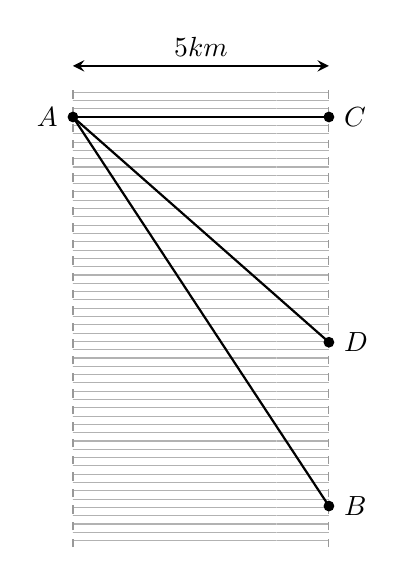
\begin{tikzpicture}[>=stealth, scale=1.3]

    % =================================================================
    % 1. ĐỊNH NGHĨA TỌA ĐỘ CÁC ĐIỂM CHÍNH
    % =================================================================
    \coordinate (A) at (0,4.0);
    \coordinate (C) at (2.5,4.0);
    \coordinate (D) at (2.5,1.8);
    \coordinate (B) at (2.5,0.2);

    % Tọa độ giới hạn vùng background gạch ngang (dòng sông/biển)
    \coordinate (TopLeftBg) at (0,4.3);
    \coordinate (TopRightBg) at (2.5,4.3);
    \coordinate (BottomLeftBg) at (0,-0.2);
    \coordinate (BottomRightBg) at (2.5,-0.2);

    % =================================================================
    % 2. TÔ VÙNG HỌA TIẾT NỀN GẠCH NGANG (DÒNG SÔNG) VÀ BIÊN NÉT ĐỨT
    % =================================================================
    % Sử dụng họa tiết nằm ngang mờ mờ làm nền cho dòng sông
    \fill[pattern=horizontal lines, pattern color=gray!60] (BottomLeftBg) rectangle (TopRightBg);
    
    % Hai đường biên dọc thể hiện hai bờ sông (nét đứt mỏng)
    \draw[dashed, gray!80, thin] (BottomLeftBg) -- (TopLeftBg);
    \draw[dashed, gray!80, thin] (BottomRightBg) -- (TopRightBg);

    % =================================================================
    % 3. VẼ CÁC TUYẾN ĐƯỜNG NỐI VÀ CÁC ĐIỂM NÚT
    % =================================================================
    % Vẽ các đoạn thẳng nối giữa các điểm
    \draw[thick] (A) -- (C);
    \draw[thick] (A) -- (D);
    \draw[thick] (A) -- (B);

    % Vẽ các chấm tròn đen tại các điểm nút đầu mút
    \fill (A) circle (1.5pt);
    \fill (C) circle (1.5pt);
    \fill (D) circle (1.5pt);
    \fill (B) circle (1.5pt);

    % =================================================================
    % 4. GÁN NHÃN ĐỈNH VÀ ĐIỀN THÔNG SỐ CHIỀU RỘNG SÔNG
    % =================================================================
    % Nhãn các điểm
    \node[left=2pt] at (A) {$A$};
    \node[right=2pt] at (C) {$C$};
    \node[right=2pt] at (D) {$D$};
    \node[right=2pt] at (B) {$B$};

    % Mũi tên kích thước thể hiện chiều rộng sông 5km phía trên
    \draw[<->, thick] (0,4.5) -- (2.5,4.5);
    \node[above] at (1.25,4.5) {$5km$};

\end{tikzpicture}
\end{center}
}{
    \textbf{a)} & \( 11 - x \) (km) là độ dài quãng đường \( BD \).
    & \textcolor{amberorange}{$\bigcirc$} & \textcolor{amberorange}{$\bigcirc$} \\ \hline
    
    \textbf{b)} & Thời gian chèo thuyền trên quãng đường \( AD \) là  
    \(\dfrac{\sqrt{25 + x^2}}{5} \text{ (giờ)}.\)
    & \textcolor{amberorange}{$\bigcirc$} & \textcolor{amberorange}{$\bigcirc$} \\ \hline
    
    \textbf{c)} & Tổng thời gian di chuyển từ \( A \) đến \( B \) là  
    \(\dfrac{\sqrt{(11 - x)^2 + 25}}{5} + \dfrac{x}{9} \text{ (giờ)}.\)
    & \textcolor{amberorange}{$\bigcirc$} & \textcolor{amberorange}{$\bigcirc$} \\ \hline
    
    \textbf{d)} & \( D \) cần cách \( B \) một khoảng 7,66 km thì tổng thời gian di chuyển từ \( A \) đến \( B \) là nhỏ nhất (kết quả làm tròn đến hàng phần trăm).
    & \textcolor{amberorange}{$\bigcirc$} & \textcolor{amberorange}{$\bigcirc$} \\
}

% --- CÂU 6 ---
\questionTrueFalse{0}{6}{Một khu vui chơi trẻ em có hai cây cột, cây thứ nhất cao 15m và cây thứ hai cao 30m đứng cách nhau 80m. Chúng được giữ bằng hai sợi dây, gắn vào một cọc duy nhất nối từ mặt đất đến đỉnh mỗi cột (như hình vẽ). Gọi \( x \) là khoảng cách từ cây thứ nhất đến cọc (đơn vị: mét), \( 0 < x < 80 \).
\begin{center}
    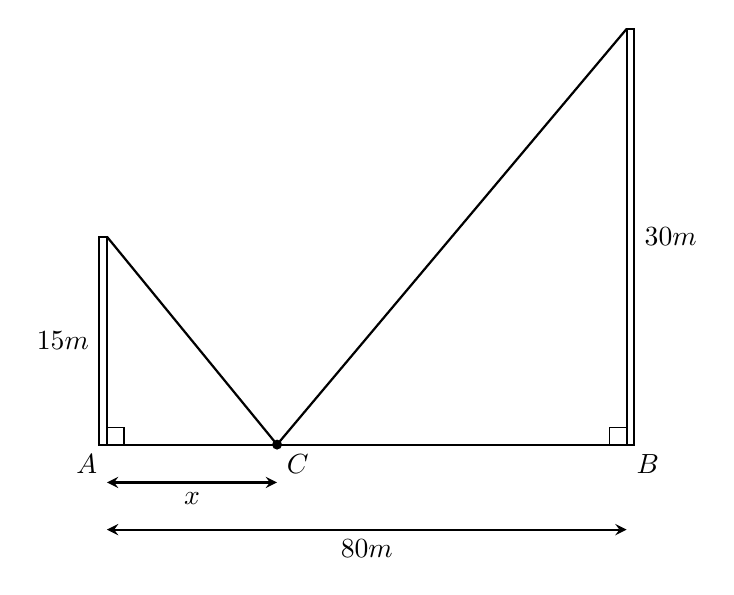
\begin{tikzpicture}[>=stealth, scale=1.2]

    % =================================================================
    % 1. ĐỊNH NGHĨA TỌA ĐỘ CÁC ĐIỂM CHÍNH
    % =================================================================
    \coordinate (A) at (0,0);
    \coordinate (B) at (5.5,0);
    \coordinate (C) at (1.8,0);
    
    % Hai đỉnh cột (vẽ dạng cột mỏng hình chữ nhật)
    \coordinate (TopA) at (0,2.2);
    \coordinate (TopB) at (5.5,4.4);

    % =================================================================
    % 2. VẼ ĐƯỜNG MẶT ĐẤT VÀ CÁC SỢI DÂY NỐI
    % =================================================================
    % Đường mặt đất nằm ngang nối từ A đến B
    \draw[thick] (A) -- (B);

    % Hai sợi dây căng từ đỉnh cột xuống điểm C trên mặt đất
    \draw[thick] (TopA) -- (C);
    \draw[thick] (TopB) -- (C);

    % =================================================================
    % 3. VẼ HAI CỘT ĐỨNG (CÓ ĐỘ DÀY NHẸ NHƯ HÌNH GỐC)
    % =================================================================
    \draw[thick, fill=white] (-0.08,0) rectangle (0,2.2);
    \draw[thick, fill=white] (5.5,0) rectangle (5.58,4.4);

    % =================================================================
    % 4. VẼ CÁC KÝ HIỆU GÓC VUÔNG VÀ CHẤM TRÒN TẠI C
    % =================================================================
    % Góc vuông tại gốc cột A (nằm bên phải cột)
    \draw[thin] (A) ++(0,0.18) -- ++(0.18,0) -- ++(0,-0.18);
    
    % Góc vuông tại gốc cột B (nằm bên trái cột)
    \draw[thin] (B) ++(0,0.18) -- ++(-0.18,0) -- ++(0,-0.18);

    % Chấm tròn đen tại điểm C
    \fill (C) circle (1.5pt);

    % =================================================================
    % 5. GÁN NHÃN ĐỈNH VÀ THÔNG SỐ ĐỘ DÀI
    % =================================================================
    % Tên các điểm trên mặt đất
    \node[below left] at (A) {$A$};
    \node[below right] at (B) {$B$};
    \node[below right] at (C) {$C$};

    % Chiều cao của hai cột
    \node[left=3pt] at (0,1.1) {$15m$};
    \node[right=3pt] at (5.5,2.2) {$30m$};

    % =================================================================
    % 6. VẼ HỆ THỐNG MŨI TÊN KÍCH THƯỚC PHÍA DƯỚI
    % =================================================================
    % Khoảng cách x (từ A đến C)
    \draw[<->, thick] (0,-0.4) -- (1.8,-0.4);
    \node[below] at (0.9,-0.4) {$x$};

    % Tổng khoảng cách 80m (từ A đến B)
    \draw[<->, thick] (0,-0.9) -- (5.5,-0.9);
    \node[below] at (2.75,-0.9) {$80m$};

\end{tikzpicture}
\end{center}
}{
    \textbf{a)} & Chiều dài sợi dây nối từ cọc đến đỉnh cây thứ hai là  
    \[\sqrt{30 + (x - 80)^2} \, \text{mét.}\]
    & \textcolor{amberorange}{$\bigcirc$} & \textcolor{amberorange}{$\bigcirc$} \\ \hline
    
    \textbf{b)} & Tổng chiều dài sợi dây nối từ cọc đến hai đỉnh của hai cây là  
    \[\sqrt{x^2 + 15} + \sqrt{30 + (80 - x)^2} \, \text{mét.}\]
    & \textcolor{amberorange}{$\bigcirc$} & \textcolor{amberorange}{$\bigcirc$} \\ \hline
    
    \textbf{c)} & Để tổng chiều dài sợi dây ngắn nhất thì \( x \in (0; 35) \).
    & \textcolor{amberorange}{$\bigcirc$} & \textcolor{amberorange}{$\bigcirc$} \\ \hline
    
    \textbf{d)} & Tổng chiều dài ngắn nhất của dây xấp xỉ 92 km.
    & \textcolor{amberorange}{$\bigcirc$} & \textcolor{amberorange}{$\bigcirc$} \\
}

% --- CÂU 7 ---
\questionTrueFalse{0}{7}{Có hai người đi ô tô ở hai vị trí A và B. Người ở vị trí A lái xe theo hướng Nam đến vị trí C với vận tốc 60 km/h, còn người ở vị trí B lái xe với vận tốc 45 km/h để đến vị trí D (như hình vẽ). Biết rằng \( AB = 80 \, \text{km} \). Gọi \( t \) (giờ) là thời gian lái xe của mỗi người.
\begin{center}
    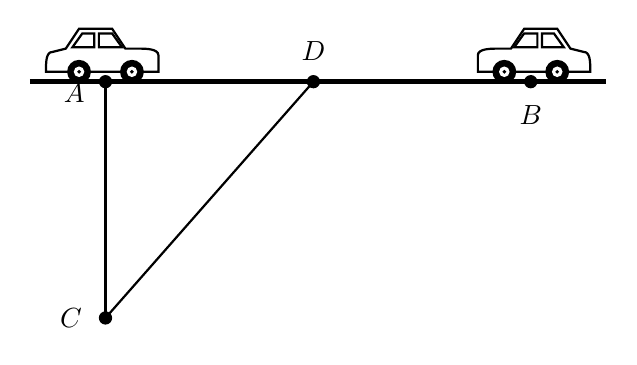
\begin{tikzpicture}[>=stealth, scale=1.2]

    % =================================================================
    % 1. ĐỊNH NGHĨA TỌA ĐỘ CÁC ĐIỂM CHÍNH
    % =================================================================
    \coordinate (A) at (0,2.5);
    \coordinate (B) at (4.5,2.5);
    \coordinate (D) at (2.2,2.5);
    \coordinate (C) at (0,0);
    
    % Giới hạn hai đầu đường lộ
    \coordinate (RoadStart) at (-0.8,2.5);
    \coordinate (RoadEnd) at (5.3,2.5);

    % =================================================================
    % 2. VẼ ĐƯỜNG LỘ VÀ CÁC TUYẾN ĐƯỜNG NỐI
    % =================================================================
    % Đường nằm ngang (mặt đường lộ)
    \draw[ultra thick] (RoadStart) -- (RoadEnd);

    % Các đoạn thẳng nối AC và CD
    \draw[thick] (A) -- (C);
    \draw[thick] (C) -- (D);

    % =================================================================
    % 3. VẼ CÁC ĐIỂM NÚT (CHẤM TRÒN ĐEN)
    % =================================================================
    \fill (A) circle (2pt);
    \fill (B) circle (2pt);
    \fill (C) circle (2pt);
    \fill (D) circle (2pt);

    % =================================================================
    % 4. ĐỊNH NGHĨA HÀM VẼ XE Ô TÔ CÓ THỂ QUAY HƯỚNG (XSCALE)
    % =================================================================
    % #1: Vị trí đặt xe (A hoặc B)
    % #2: Hướng đầu xe (1: hướng sang phải, -1: hướng sang trái)
    \newcommand{\drawcar}[2]{
        \begin{scope}[shift={#1}, scale=0.7, xscale=#2]
            % Thân xe dưới
            \draw[thick, fill=white] (-0.8, 0.15) 
                -- (-0.8, 0.4) 
                .. controls (-0.8, 0.5) and (-0.6, 0.5) .. (-0.5, 0.5) % Đuôi xe
                -- (-0.3, 0.5)
                -- (-0.1, 0.8) % Kính sau
                -- (0.4, 0.8)  % Mui xe
                -- (0.6, 0.5)  % Kính trước
                -- (0.8, 0.45) % Đầu xe
                .. controls (0.9, 0.45) and (0.9, 0.3) .. (0.9, 0.15)
                -- cycle;
            
            % Cửa sổ xe
            \draw[thick, fill=white] (-0.25, 0.52) -- (-0.1, 0.73) -- (0.1, 0.73) -- (0.1, 0.52) -- cycle;
            \draw[thick, fill=white] (0.17, 0.52) -- (0.17, 0.73) -- (0.35, 0.73) -- (0.5, 0.52) -- cycle;

            % Bánh xe trước & sau (Hình tròn đồng tâm tạo lốp và vành)
            \fill[black] (-0.4, 0.15) circle (0.18);
            \fill[white] (-0.4, 0.15) circle (0.08);
            \fill[black] (-0.4, 0.15) circle (0.03);
            
            \fill[black] (0.4, 0.15) circle (0.18);
            \fill[white] (0.4, 0.15) circle (0.08);
            \fill[black] (0.4, 0.15) circle (0.03);
        \end{scope}
    }

    % Vẽ xe tại vị trí A (Đầu xe hướng sang phải)
    \drawcar{(A)}{-1};
    
    % Vẽ xe tại vị trí B (Đầu xe hướng sang trái - quay đầu về phía điểm D)
    \drawcar{(B)}{1};

    % =================================================================
    % 5. GÁN NHÃN CÁC ĐIỂM
    % =================================================================
    \node[left=4pt, yshift=-4pt] at (A) {$A$};
    \node[below=5pt] at (B) {$B$};
    \node[left=5pt] at (C) {$C$};
    \node[above=4pt] at (D) {$D$};

\end{tikzpicture}
\end{center}
}{
    \textbf{a)} & Quãng đường người ở vị trí A đi được sau \( t \) giờ là \( 60t \, (\text{km}) \).
    & \textcolor{amberorange}{$\bigcirc$} & \textcolor{amberorange}{$\bigcirc$} \\ \hline
    
    \textbf{b)} & Quãng đường người ở vị trí B đi được sau \( t \) giờ là \( 45t \, (\text{km}) \).
    & \textcolor{amberorange}{$\bigcirc$} & \textcolor{amberorange}{$\bigcirc$} \\ \hline
    
    \textbf{c)} & Độ dài đoạn \( CD \) tính theo \( t \) là  
    \(\sqrt{60t^2 + 45(80 - t)^2} \, (\text{km}).\)
    & \textcolor{amberorange}{$\bigcirc$} & \textcolor{amberorange}{$\bigcirc$} \\ \hline
    
    \textbf{d)} & Khi hai người cách nhau một khoảng ngắn nhất thì thời gian đi của mỗi người là 50 phút.
    & \textcolor{amberorange}{$\bigcirc$} & \textcolor{amberorange}{$\bigcirc$} \\
}

% --- CÂU 8 ---
\questionTrueFalse{0}{8}{Một ngọn hải đăng được đặt tại vị trí A cách bờ biển một khoảng \( AB = 10 \, km \). Trên bờ biển có một cảng thuyền ở vị trí C cách B một khoảng \( BC = 18 \, km \) (tham khảo hình vẽ). Người canh hải đăng có thể chèo thuyền từ vị trí A đến M với vận tốc 6 km/h và đi xe điện từ vị trí M đến cảng C với vận tốc 15 km/h. Đặt \( BM = x \) (\( 0 < x < 12 \)).
\begin{center}
    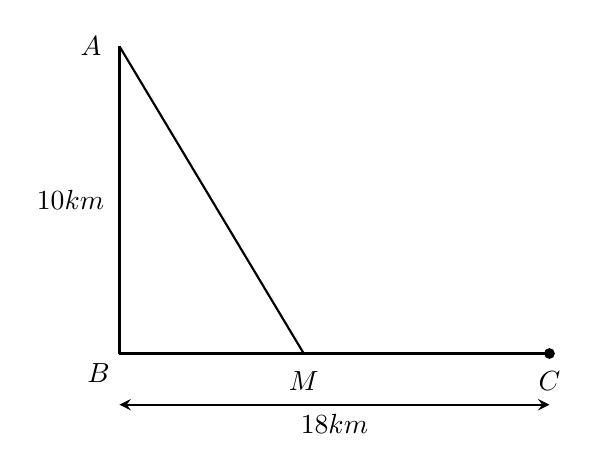
\begin{tikzpicture}[>=stealth, scale=1.3]

    % =================================================================
    % 1. ĐỊNH NGHĨA TỌA ĐỘ CÁC ĐIỂM CHÍNH
    % =================================================================
    \coordinate (B) at (0,0);
    \coordinate (M) at (1.8,0);
    \coordinate (C) at (4.2,0);
    \coordinate (A) at (0,3.0);

    % =================================================================
    % 2. VẼ CÁC ĐƯỜNG THẲNG
    % =================================================================
    % Đường nằm ngang BC
    \draw[thick] (B) -- (C);

    % Đoạn thẳng đứng AB và đoạn thẳng nghiêng AM
    \draw[thick] (A) -- (B);
    \draw[thick] (A) -- (M);

    % Điểm C được biểu diễn bằng một chấm tròn đen nhỏ ở đầu mút
    \fill (C) circle (1.5pt);

    % =================================================================
    % 3. GÁN NHÃN CÁC ĐỈNH VÀ THÔNG SỐ ĐỘ DÀI
    % =================================================================
    \node[left=3pt] at (A) {$A$};
    \node[below left] at (B) {$B$};
    \node[below=3pt] at (M) {$M$};
    \node[below=3pt] at (C) {$C$};

    % Thông số độ dài đoạn AB
    \node[left=2pt] at (0,1.5) {$10km$};

    % =================================================================
    % 4. VẼ MŨI TÊN KÍCH THƯỚC CHIỀU DÀI 18km PHÍA DƯỚI
    % =================================================================
    \draw[<->, thick] (0,-0.5) -- (4.2,-0.5);
    \node[below] at (2.1,-0.5) {$18km$};

\end{tikzpicture}
\end{center}
}{
    \textbf{a)} & Thời gian đi từ A đến M là \( 6\sqrt{x^2 + 100} \) giờ.
    & \textcolor{amberorange}{$\bigcirc$} & \textcolor{amberorange}{$\bigcirc$} \\ \hline
    
    \textbf{b)} & Thời gian đi từ A đến C là \( 6\sqrt{x^2 + 100} + 15(18 - x) \) giờ.
    & \textcolor{amberorange}{$\bigcirc$} & \textcolor{amberorange}{$\bigcirc$} \\ \hline
    
    \textbf{c)} & Khi thời gian người đó đến C ngắn nhất thì \( MB = \dfrac{20}{\sqrt{21}} \, km \).
    & \textcolor{amberorange}{$\bigcirc$} & \textcolor{amberorange}{$\bigcirc$} \\ \hline
    
    \textbf{d)} & Để người đó đến C đúng vào lúc 7h sáng thì người đó phải xuất phát từ vị trí A muộn nhất lúc 4h23p.
    & \textcolor{amberorange}{$\bigcirc$} & \textcolor{amberorange}{$\bigcirc$} \\
}

% --- CÂU 9 ---
\questionShortAnswer{0}{9}{Một đường nước sạch được nối từ một nhà máy nước ở \( A \) (nằm tại bờ biển là đường thẳng \( AB \)) đến một hòn đảo \( C \), khoảng cách ngắn nhất từ đảo về bờ biển là đoạn \( BC \) dài \( 12 \, \text{km} \), khoảng cách từ \( B \) đến \( A \) dài \( 40 \, \text{km} \) được minh họa bằng hình vẽ dưới đây.

\begin{center}
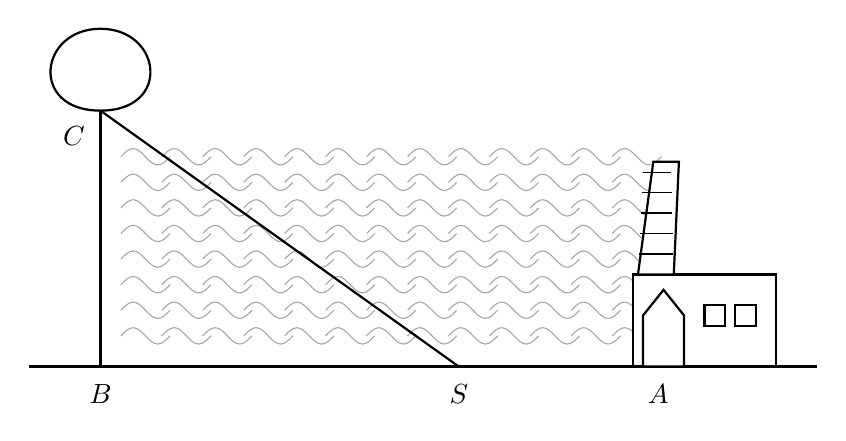
\begin{tikzpicture}[>=stealth, scale=1.3]

    % =================================================================
    % 1. ĐỊNH NGHĨA TỌA ĐỘ CÁC ĐIỂM CHÍNH
    % =================================================================
    \coordinate (B) at (0,0);
    \coordinate (S) at (3.5,0);
    \coordinate (A) at (5.2,0);
    \coordinate (C) at (0,2.5);
    
    % Giới hạn trục nằm ngang mặt đất
    \coordinate (GroundStart) at (-0.7,0);
    \coordinate (GroundEnd) at (7.0,0);

    % =================================================================
    % 2. VẼ NỀN SÓNG NƯỚC (DÒNG SÔNG)
    % =================================================================
    % Điền các ký hiệu sóng nước mờ lặp lại dạng cột để minh họa dòng sông
    \foreach \x in {0.2, 0.6, 1.0, 1.4, 1.8, 2.2, 2.6, 3.0, 3.4, 3.8, 4.2, 4.6, 5.0} {
        \foreach \y in {0.3, 0.55, 0.8, 1.05, 1.3, 1.55, 1.8, 2.05} {
            \draw[shift={(\x,\y)}, xscale=0.6, yscale=0.4, thin, gray!70] 
                (0,0) sin (0.2,0.2) cos (0.4,0) sin (0.6,-0.2) cos (0.8,0);
        }
    }

    % =================================================================
    % 3. VẼ ĐƯỜNG MẶT ĐẤT VÀ CÁC ĐOẠN THẲNG TRONG BÀI TOÁN
    % =================================================================
    % Đường mặt đất nằm ngang
    \draw[thick] (GroundStart) -- (GroundEnd);

    % Đoạn thẳng đứng BC (chiều cao khinh khí cầu) và đường nhìn nghiêng CS
    \draw[thick] (B) -- (C);
    \draw[thick] (C) -- (S);

    % =================================================================
    % 4. VẼ KHINH KHÍ CẦU VÀ NGÔI NHÀ/NHÀ MÁY
    % =================================================================
    % Vẽ khinh khí cầu tại đỉnh C
    \draw[thick, fill=white] (C) .. controls (-0.7, 2.5) and (-0.6, 3.3) .. (0, 3.3)
                             .. controls (0.6, 3.3) and (0.7, 2.5) .. (C) -- cycle;

    % Vẽ ngôi nhà / nhà máy bên phải điểm A
    \begin{scope}[shift={(A)}]
        % Thân nhà chính
        \draw[thick, fill=white] (0,0) rectangle (1.4, 0.9);
        % Cửa ra vào lớn hình vòm nhọn
        \draw[thick, fill=white] (0.1, 0) -- (0.1, 0.5) -- (0.3, 0.75) -- (0.5, 0.5) -- (0.5, 0) -- cycle;
        % Cửa sổ nhỏ vuông bên phải
        \draw[thick] (0.7, 0.4) rectangle (0.9, 0.6);
        \draw[thick] (1.0, 0.4) rectangle (1.2, 0.6);
        % Ống khói cao chia thành từng đốt tầng
        \draw[thick, fill=white] (0.05, 0.9) -- (0.2, 2.0) -- (0.45, 2.0) -- (0.4, 0.9) -- cycle;
        \foreach \h in {1.1, 1.3, 1.5, 1.7, 1.9} {
            \draw[thin] (0.05+\h*0.06-0.06, \h) -- (0.4-\h*0.03+0.03, \h);
        }
    \end{scope}

    % =================================================================
    % 5. GÁN NHÃN ĐỈNH VÀ ĐIỂM
    % =================================================================
    \node[below=3pt] at (B) {$B$};
    \node[below=3pt] at (S) {$S$};
    \node[below=3pt] at (5.45, 0) {$A$};
    \node[below left=3pt] at (C) {$C$};

\end{tikzpicture}
\end{center}

Biết rằng mỗi \( km \) đường ống đặt dưới nước chi phí mất \( 500 \, 000 \, \text{đồng} \), còn đặt dưới đất chi phí mất \( 300 \, 000 \, \text{đồng} \). Chi phí thấp nhất cần bỏ ra để lắp đặt đường ống từ nhà máy \( A \) đến đảo \( C \) là bao nhiêu triệu đồng?}

% --- CÂU 10 ---
\questionShortAnswer{0}{10}{Một người đưa thư đang ở điểm \( A \), cách điểm \( B \) một đoạn đường xuyên rừng dài \( 60 \, \text{km} \). Trong rừng, người này chỉ có thể di chuyển với vận tốc \( 25 \, \text{km/h} \), và người này cần đến \( B \) trong tối đa \( 2,25 \, \text{giờ} \). May mắn thay, có một con đường nhựa cách đoạn \( AB \) một khoảng \( 12 \, \text{km} \), chạy song song với nó. Trên đường nhựa, người này có thể di chuyển với vận tốc \( 45 \, \text{km/h} \). Biết rằng, nếu di chuyển trên đường nhựa thì người đó sẽ đi theo đường gấp khúc dạng hình thang cân \( ACDB \). Hỏi thời gian ngắn nhất để người đưa thư đi từ \( A \) đến \( B \) là bao nhiêu giờ (kết quả làm tròn đến hàng phần trăm)?

\begin{center}
\begin{tikzpicture}[>=stealth, scale=1.3]

    % =================================================================
    % 1. ĐỊNH NGHĨA TỌA ĐỘ CÁC ĐIỂM CHÍNH
    % =================================================================
    \coordinate (A) at (0,0);
    \coordinate (B) at (6.0,0);
    \coordinate (C) at (1.2,2.5);
    \coordinate (D) at (4.8,2.5);
    
    % Các đỉnh phụ để vẽ đường nét đứt thể hiện chiều cao hình thang
    \coordinate (TopA) at (0,2.5);
    \coordinate (TopB) at (6.0,2.5);
    
    % Giới hạn trục nằm ngang phía dưới
    \coordinate (LineStart) at (-0.7,0);
    \coordinate (LineEnd) at (6.7,0);

    % =================================================================
    % 2. VẼ CÁC ĐƯỜNG THẲNG LIỀN NÉT VÀ NÉT ĐỨT
    % =================================================================
    % Đường nền nằm ngang phía dưới đi qua A và B
    \draw[thick] (LineStart) -- (LineEnd);

    % Đường nhựa nằm ngang phía trên (bao gồm cả các đoạn kéo dài sang hai bên)
    \draw[thick] (TopA) -- (TopB);

    % Hai đường xiên AC và BD
    \draw[thick] (A) -- (C);
    \draw[thick] (B) -- (D);

    % Hai đoạn thẳng đứng thể hiện chiều cao vuông góc (nét đứt)
    \draw[dashed, thick] (A) -- (TopA);
    \draw[dashed, thick] (B) -- (TopB);

    % =================================================================
    % 3. VẼ CÁC ĐIỂM NÚT (CHẤM TRÒN ĐEN)
    % =================================================================
    \fill (A) circle (1.8pt);
    \fill (B) circle (1.8pt);
    \fill (C) circle (1.8pt);
    \fill (D) circle (1.8pt);

    % =================================================================
    % 4. GÁN NHÃN ĐỈNH VÀ ĐIỀN CHÚ THÍCH CHỮ
    % =================================================================
    % Nhãn các điểm hình học
    \node[below left] at (A) {$A$};
    \node[below right] at (B) {$B$};
    \node[above left] at (C) {$C$};
    \node[above right] at (D) {$D$};

    % Thông số khoảng cách/chiều cao 12km
    \node[left=3pt] at (0,1.25) {$12km$};

    % Các nhãn văn bản chú thích địa hình
    \node[above] at (3.0, 2.5) {Đường nhựa};
    \node at (3.0, 1.2) {Rừng};
    \node[below] at (3.0, -0.1) {Rừng};

\end{tikzpicture}
\end{center}}

% --- CÂU 11 ---
\questionShortAnswer{0}{11}{Hai trạm thu phát sóng ở hai vị trí \( A \) và \( B \) nằm về hai phía của một thung lũng. Trạm \( A \) cách thung lũng một khoảng là \( 3 \, \text{km} \), trạm \( B \) cách thung lũng một khoảng là \( 5 \, \text{km} \). Một tuyến cáp quang \( EF \) được thiết kế nối hai điểm đối diện nhau trên bờ thung lũng sao cho \( HE + KF = 15 \, \text{km} \) và độ dài \( EF \) không đổi (được mô hình hóa như hình vẽ bên dưới). Hỏi độ dài \( EH \) là bao nhiêu \( km \) để đường đi từ thành phố \( A \) đến thành phố \( B \) là ngắn nhất (đi theo đường \( AEFB \)) (kết quả làm tròn đến hàng phần trăm)?

\begin{center}
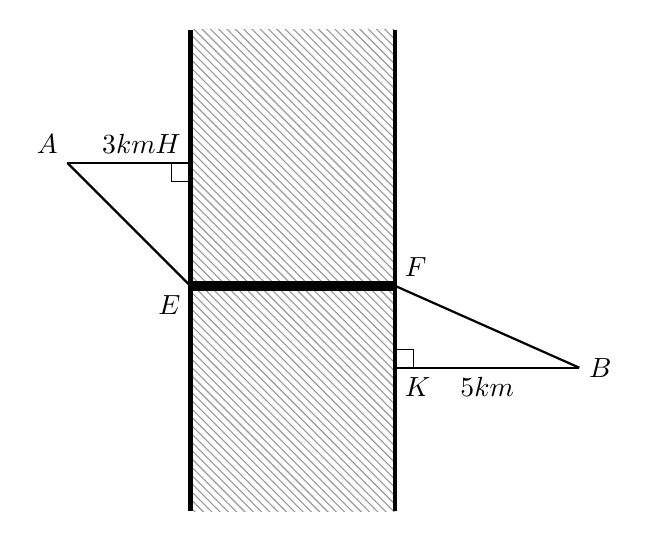
\begin{tikzpicture}[>=stealth, scale=1.3]

    % =================================================================
    % 1. ĐỊNH NGHĨA TỌA ĐỘ CÁC ĐIỂM CHÍNH
    % =================================================================
    \coordinate (H) at (0,1.2);
    \coordinate (E) at (0,0);
    \coordinate (A) at (-1.2,1.2);
    
    \coordinate (F) at (2.0,0);
    \coordinate (K) at (2.0,-0.8);
    \coordinate (B) at (3.8,-0.8);

    % Giới hạn trục dọc hai bờ sông/kênh
    \coordinate (LeftTop) at (0,2.5);
    \coordinate (LeftBottom) at (0,-2.2);
    \coordinate (RightTop) at (2.0,2.5);
    \coordinate (RightBottom) at (2.0,-2.2);

    % =================================================================
    % 2. TÔ VÙNG HỌA TIẾT NỀN GẠCH CHÉO (DÒNG SÔNG) VÀ BIÊN DỌC
    % =================================================================
    % Điền họa tiết gạch chéo xiên làm nền
    \fill[pattern=north west lines, pattern color=gray!80] (LeftBottom) rectangle (RightTop);
    
    % Hai đường biên dọc thể hiện hai bờ sông
    \draw[ultra thick] (LeftBottom) -- (LeftTop);
    \draw[ultra thick] (RightBottom) -- (RightTop);

    % =================================================================
    % 3. VẼ CÁC TUYẾN ĐƯỜNG NỐI VÀ ĐOẠN ĐƯỜNG ĐI LẠI
    % =================================================================
    % Đoạn nằm ngang AH và KB
    \draw[thick] (A) -- (H);
    \draw[thick] (K) -- (B);

    % Đoạn xiên AE và FB
    \draw[thick] (A) -- (E);
    \draw[thick] (F) -- (B);

    % Đoạn cầu nối nằm ngang vuông góc EF (vẽ nét siêu đậm nổi bật trên nền)
    \draw[line width=3.5pt] (E) -- (F);

    % =================================================================
    % 4. VẼ KÝ HIỆU GÓC VUÔNG TẠI H VÀ K
    % =================================================================
    % Góc vuông dưới điểm H
    \draw[thin] (H) ++(0,-0.18) -- ++(-0.18,0) -- ++(0,0.18);
    
    % Góc vuông trên điểm K
    \draw[thin] (K) ++(0,0.18) -- ++(0.18,0) -- ++(0,-0.18);

    % =================================================================
    % 5. GÁN NHÃN ĐỈNH VÀ ĐIỀN THÔNG SỐ KÍCH THƯỚC
    % =================================================================
    % Tên các điểm hình học
    \node[above left] at (A) {$A$};
    \node[above left] at (H) {$H$};
    \node[below left] at (E) {$E$};
    \node[above right] at (F) {$F$};
    \node[below right] at (K) {$K$};
    \node[right] at (B) {$B$};

    % Thông số độ dài khoảng cách
    \node[above] at (-0.6,1.2) {$3km$};
    \node[below] at (2.9,-0.8) {$5km$};

\end{tikzpicture}
\end{center}}

% --- CÂU 12 ---
\questionShortAnswer{0}{12}{Một kỹ sư đang thiết kế một đường ống dẫn để vận chuyển dầu thô từ mỏ dầu \( A \) cách bờ biển 6 km đến cảng xuất khẩu \( B \). Đường ống có thể nối trực tiếp từ \( A \) đến \( B \) hoặc nối từ \( A \) đến một điểm trung chuyển \( D \) trên đoạn \( BC \), rồi tiếp tục nối từ \( D \) đến \( B \). Biết khoảng cách \( BC = 10 \, km \); chi phí lắp đặt mỗi km đường ống trên biển và trên đất liền tương ứng bằng 20 và 4 (đơn vị: triệu USD). Chi phí lắp đặt đường ống thấp nhất là bao nhiêu triệu USD (kết quả làm tròn đến hàng đơn vị)?

\begin{center}
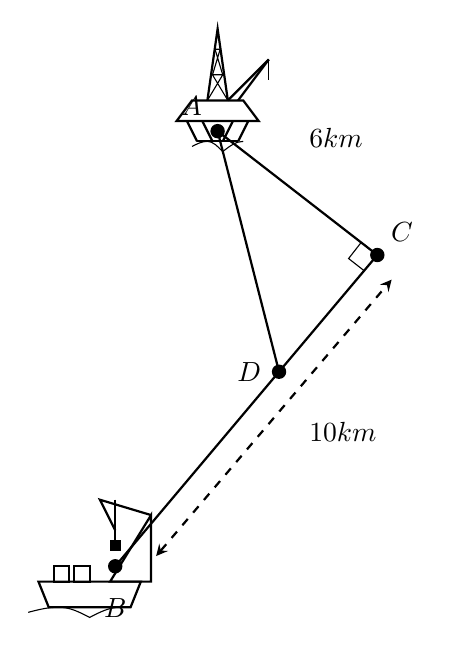
\begin{tikzpicture}[>=stealth, scale=1.3]

    % =================================================================
    % 1. ĐỊNH NGHĨA TỌA ĐỘ CÁC ĐIỂM CHÍNH (Xoay góc xiên ~ 50 độ)
    % =================================================================
    \coordinate (B) at (0,0);
    \coordinate (D) at (1.6,1.9);
    \coordinate (C) at (2.56,3.04);
    \coordinate (A) at (1.0,4.25);

    % =================================================================
    % 2. VẼ CÁC ĐOẠN THẲNG HÌNH HỌC VÀ CÁC ĐIỂM NÚT
    % =================================================================
    % Đường xiên dọc chính nối liền từ cảng B qua D đến C
    \draw[thick] (B) -- (C);

    % Các đoạn nối từ giàn khoan A đến C và D
    \draw[thick] (A) -- (C);
    \draw[thick] (A) -- (D);

    % Vẽ các chấm tròn đen lớn tại các nút đầu mút hình học
    \fill (B) circle (2pt);
    \fill (D) circle (2pt);
    \fill (C) circle (2pt);
    \fill (A) circle (2pt);

    % =================================================================
    % 3. VẼ KÝ HIỆU GÓC VUÔNG TẠI C (Vuông góc góc dưới bên trái)
    % =================================================================
    \begin{scope}[shift={(C)}, rotate=-38]
        \draw[thin] (0,0) -- (-0.2,0) -- (-0.2,-0.2) -- (0,-0.2);
    \end{scope}

    % =================================================================
    % 4. VẼ BIỂU TƯỢNG VECTOR (GIÀN KHOAN A & BẰNG PHẲNG CẢNG B)
    % =================================================================
    % Đồ họa giàn khoan A (Phía trên)
    \begin{scope}[shift={(A)}, scale=0.5, yshift=0.2cm]
        \draw[thick, fill=white] (-0.8,0) -- (0.8,0) -- (0.5,0.4) -- (-0.5,0.4) -- cycle;
        \draw[thick] (-0.6,0) -- (-0.4,-0.4) (-0.3,0) -- (-0.1,-0.4) (0.3,0) -- (0.1,-0.4) (0.6,0) -- (0.4,-0.4);
        \draw[thick] (-0.4,-0.4) -- (0.4,-0.4);
        \draw[thin] (-0.5,-0.5) sin (-0.2,-0.4) cos (0.1,-0.6) sin (0.5,-0.4);
        % Tháp khoan
        \draw[thick] (-0.2,0.4) -- (0,1.8) -- (0.2,0.4);
        \draw[thin] (-0.1,0.9) -- (0.1,0.9) (-0.05,1.4) -- (0.05,1.4);
        \draw[thin] (-0.2,0.4) -- (0.1,0.9) -- (-0.1,0.9) -- (0.2,0.4);
        \draw[thin] (-0.1,0.9) -- (0.05,1.4) -- (-0.05,1.4) -- (0.1,0.9);
        % Cần cẩu
        \draw[thick] (0.2,0.4) -- (1.0,1.2);
        \draw[thick] (0.4,0.4) -- (1.0,1.2);
        \draw[thin] (1.0,1.2) -- (1.0,0.8);
    \end{scope}

    % Đồ họa tàu thuyền và cần cẩu cảng B (Phía dưới)
    \begin{scope}[shift={(B)}, scale=0.5, xshift=-0.5cm, yshift=-0.5cm]
        % Chiếc tàu thủy
        \draw[thick, fill=white] (-1.0,0.2) -- (1.0,0.2) -- (0.8,-0.3) -- (-0.8,-0.3) -- cycle;
        \draw[thin] (-1.2,-0.4) sin (-0.6,-0.3) cos (0,-0.5) sin (0.6,-0.3);
        \draw[thick] (-0.7,0.2) rectangle (-0.4,0.5);
        \draw[thick] (-0.3,0.2) rectangle (0.0,0.5);
        % Cần cẩu bờ kè
        \draw[thick] (0.4,0.2) -- (1.2,0.2) -- (1.2,1.5) -- cycle;
        \draw[thick] (1.2,1.5) -- (0.2,1.8) -- (0.5,1.2);
        \draw[thick] (0.5,1.8) -- (0.5,1.0);
        \draw[fill=black] (0.4,0.8) rectangle (0.6,1.0);
    \end{scope}

    % =================================================================
    % 5. GÁN NHÃN ĐỈNH VÀ THÔNG SỐ SỐ ĐO
    % =================================================================
    \node[above left=3pt] at (A) {$A$};
    \node[below=8pt] at (B) {$B$};
    \node[left=3pt] at (D) {$D$};
    \node[above right=2pt] at (C) {$C$};

    % Đoạn 6km
    \node[above right] at (1.8,4.0) {$6km$};

    % Mũi tên nét đứt đôi biểu diễn chiều dài 10km dọc đường xiên BC
    \draw[<->, dashed, thick] (0.4,0.1) -- (2.7,2.8);
    \node[below right] at (1.8,1.5) {$10km$};

\end{tikzpicture}
\end{center}}

% --- CÂU 13 ---
\questionShortAnswer{0}{13}{Hai con tàu A và B đang ở cùng một vĩ tuyến và cách nhau 6 hải lí. Cả hai tàu đồng thời cùng khởi hành. Tàu A chạy về hướng Nam với vận tốc 5 hải lí/giờ, còn tàu B chạy về vị trí hiện tại của tàu A với vận tốc 6 hải lí/giờ. Hỏi sau bao nhiêu giờ thì khoảng cách giữa hai tàu là ngắn nhất (kết quả làm tròn đến hàng phần trăm)?
\begin{center}
    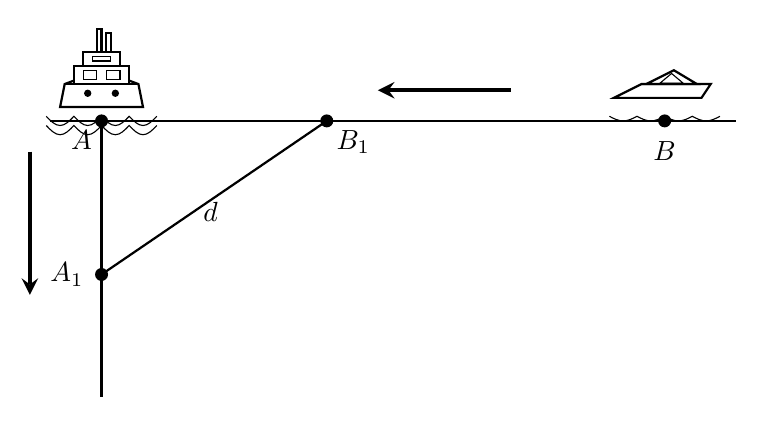
\begin{tikzpicture}[>=stealth, scale=1.3]

    % =================================================================
    % 1. ĐỊNH NGHĨA TỌA ĐỘ CÁC ĐIỂM CHÍNH
    % =================================================================
    \coordinate (A) at (0,2.5);
    \coordinate (A1) at (0,1.0);
    \coordinate (B1) at (2.2,2.5);
    \coordinate (B) at (5.5,2.5);
    
    % Các đường kéo dài biên
    \coordinate (LeftEnd) at (-0.5,2.5);
    \coordinate (RightEnd) at (6.2,2.5);
    \coordinate (BottomEnd) at (0,-0.2);

    % =================================================================
    % 2. VẼ CÁC ĐƯỜNG THẲNG LỘ TRÌNH VÀ KHOẢNG CÁCH
    % =================================================================
    % Tuyến đường nằm ngang và tuyến dọc xuống dưới
    \draw[thick] (LeftEnd) -- (RightEnd);
    \draw[thick] (A) -- (BottomEnd);

    % Đoạn thẳng nối khoảng cách d giữa A1 và B1
    \draw[thick] (A1) -- (B1);

    % =================================================================
    % 3. VẼ CÁC ĐIỂM NÚT (CHẤM TRÒN ĐEN)
    % =================================================================
    \fill (A) circle (1.8pt);
    \fill (A1) circle (1.8pt);
    \fill (B1) circle (1.8pt);
    \fill (B) circle (1.8pt);

    % =================================================================
    % 4. VẼ HÌNH VECTOR MINH HỌA CÁC CHIẾC TÀU THUYỀN
    % =================================================================
    
    % --- Tàu lớn tại vị trí A (Tàu chở hàng hướng thẳng mặt) ---
    \begin{scope}[shift={(A)}, scale=0.45, yshift=0.3cm]
        % Sóng nước dưới chân tàu lớn
        \draw[thin] (-1.2,-0.2) sin (-0.9,-0.4) cos (-0.6,-0.2) sin (-0.3,-0.4) cos (0,-0.2) 
                               sin (0.3,-0.4) cos (0.6,-0.2) sin (0.9,-0.4) cos (1.2,-0.2);
        \draw[thin] (-1.2,-0.4) sin (-0.9,-0.6) cos (-0.6,-0.4) sin (-0.3,-0.6) cos (0,-0.4) 
                               sin (0.3,-0.6) cos (0.6,-0.4) sin (0.9,-0.6) cos (1.2,-0.4);
        % Thân tàu chính
        \draw[thick, fill=white] (-0.9,0) -- (0.9,0) -- (0.8,0.5) -- (0,0.8) -- (-0.8,0.5) -- cycle;
        \draw[thick] (-0.8,0.5) -- (0.8,0.5);
        \fill (0.3,0.3) circle (0.08);
        \fill (-0.3,0.3) circle (0.08);
        % Các tầng cabin
        \draw[thick, fill=white] (-0.6,0.5) rectangle (0.6,0.9);
        \draw[thin] (-0.4,0.6) rectangle (-0.1,0.8) (0.1,0.6) rectangle (0.4,0.8);
        \draw[thick, fill=white] (-0.4,0.9) rectangle (0.4,1.2);
        \draw[thin] (-0.2,1.0) rectangle (0.2,1.1);
        % Ống khói và cột radar
        \draw[thick] (0.1,1.2) -- (0.1,1.6) -- (0.2,1.6) -- (0.2,1.2);
        \draw[thick] (-0.1,1.2) -- (-0.1,1.7) -- (0.0,1.7) -- (0.0,1.2);
    \end{scope}

    % --- Tàu cano nhỏ tại vị trí B (Hướng sang bên trái) ---
    \begin{scope}[shift={(B)}, scale=0.45, yshift=0.3cm]
        % Sóng nước chân tàu nhỏ
        \draw[thin] (-1.2,-0.2) sin (-0.9,-0.3) cos (-0.6,-0.2) sin (-0.3,-0.3) cos (0,-0.2) 
                               sin (0.3,-0.3) cos (0.6,-0.2) sin (0.9,-0.3) cos (1.2,-0.2);
        % Thân cano phóng nhanh
        \draw[thick, fill=white] (-1.1,0.2) -- (0.8,0.2) -- (1.0,0.5) -- (-0.5,0.5) -- cycle;
        % Kính chắn gió và cabin vuốt nhọn
        \draw[thick, fill=white] (-0.4,0.5) -- (0.2,0.8) -- (0.7,0.5) -- cycle;
        \draw[thin] (-0.1,0.52) -- (0.15,0.73) -- (0.4,0.52) -- cycle;
    \end{scope}

    % =================================================================
    % 5. VẼ CÁC MŨI TÊN CHỈ HƯỚNG CHUYỂN ĐỘNG
    % =================================================================
    % Mũi tên chỉ hướng dịch chuyển dọc đi xuống bên trái điểm A
    \draw[->, ultra thick] (-0.7,2.2) -- (-0.7,0.8);
    
    % Mũi tên chỉ hướng dịch chuyển ngang đi sang trái ở phía trên trục
    \draw[->, ultra thick] (4.0,2.8) -- (2.7,2.8);

    % =================================================================
    % 6. GÁN NHÃN ĐỈNH VÀ THÔNG SỐ TRÊN HÌNH vẽ
    % =================================================================
    \node[below left] at (A) {$A$};
    \node[left=3pt] at (A1) {$A_1$};
    \node[below right] at (B1) {$B_1$};
    \node[below=4pt] at (B) {$B$};
    
    % Kí hiệu đoạn d
    \node[below right] at (0.9,1.8) {$d$};

\end{tikzpicture}
\end{center}
}

% --- CÂU 14 ---
\questionShortAnswer{0}{14}{Cho một bờ hồ có dạng nửa đường tròn bán kính bằng 5 km, đường kính \( MN \) như hình vẽ sau:

\begin{center}
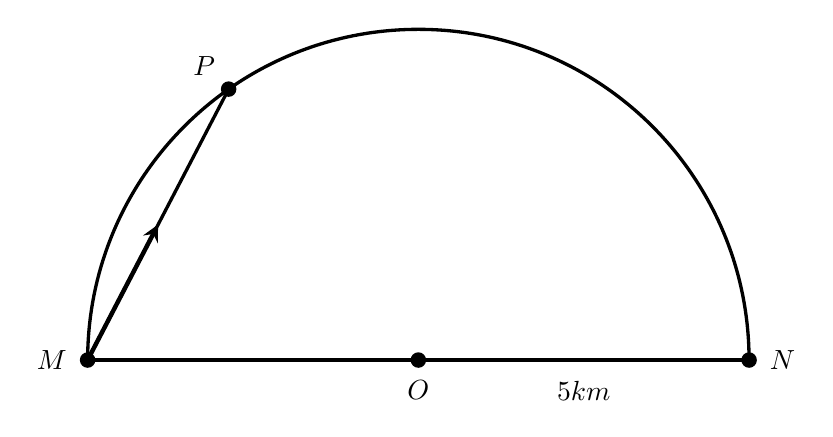
\begin{tikzpicture}[>=stealth, scale=1.4]

    % =================================================================
    % 1. ĐỊNH NGHĨA TỌA ĐỘ VÀ BÁN KÍNH ĐƯỜNG TRÒN
    % =================================================================
    % Tâm đường tròn O đặt tại gốc tọa độ (0,0), bán kính R = 3
    \coordinate (O) at (0,0);
    \coordinate (M) at (-3.0,0);
    \coordinate (N) at (3.0,0);
    
    % Điểm P nằm trên cung tròn (góc khoảng 125 độ tính từ trục Ox)
    \coordinate (P) at ({3.0*cos(125)}, {3.0*sin(125)});

    % =================================================================
    % 2. VẼ ĐƯỜNG KÍNH MN VÀ CUNG TRÒN BÁN NGUYỆT
    % =================================================================
    % Đoạn thẳng đường kính MN liền nét, dày dặn
    \draw[very thick] (M) -- (N);

    % Cung tròn nửa trên từ điểm N quay ngược chiều kim đồng hồ đến M
    \draw[very thick] (3.0,0) arc (0:180:3.0);

    % =================================================================
    % 3. VẼ TIA NỐI MP CÓ CHỨA MŨI TÊN CHỈ HƯỚNG DỊCH CHUYỂN
    % =================================================================
    % Vẽ đoạn thẳng MP
    \draw[very thick] (M) -- (P);
    
    % Vẽ mũi tên chỉ hướng nằm chính giữa đoạn thẳng MP
    \coordinate (MidMP) at ($ (M)!0.5!(P) $);
    \draw[->, ultra thick] (M) -- (MidMP);

    % =================================================================
    % 4. VẼ CÁC ĐIỂM NÚT (CHẤM TRÒN ĐEN)
    % =================================================================
    \fill (M) circle (2.0pt);
    \fill (N) circle (2.0pt);
    \fill (O) circle (2.0pt);
    \fill (P) circle (2.0pt);

    % =================================================================
    % 5. GÁN NHÃN CÁC ĐỈNH VÀ THÔNG SỐ SỐ ĐO
    % =================================================================
    \node[left=4pt] at (M) {$M$};
    \node[right=4pt] at (N) {$N$};
    \node[below=4pt] at (O) {$O$};
    \node[above left=2pt] at (P) {$P$};

    % Điền thông số chiều dài 5km bên dưới đoạn ON
    \node[below] at (1.5,-0.1) {$5km$};

\end{tikzpicture}
\end{center}

Một người Eskimo xuất phát từ điểm \( M \), trượt bằng thuyền kayak trên bảng với vận tốc 5 km/h đến điểm \( P \) trên bờ hồ, rồi chạy bộ trên bảng theo mép hồ đến điểm \( N \) với vận tốc 8 km/h. Hỏi thời gian lớn nhất người Eskimo có thể mất để đi từ \( M \) đến \( N \) là bao nhiêu (thời gian tính bằng giờ, kết quả làm tròn đến hàng phần trăm)?}

% --- CÂU 15 ---
\questionShortAnswer{0}{15}{Bạn Khoa thường đi bơi ở hồ Skylake, hồ bơi có thiết kế là một hình chữ nhật với chiều dài 30 m, chiều rộng 18 m và bên cạnh đó là một hình bán nguyệt đường kính 14 m. Trong một lần bể bơi vắng người nên Khoa đã thực hiện một chu trình là bơi theo đoạn thẳng \( AC \) rồi bơi tiếp đoạn thẳng \( CM \), với \( M \) là một vị trí bất kỳ trên hình bán nguyệt. Ngay sau đó bạn đi bộ theo một hướng qua điểm \( D \) dọc bờ của hồ bơi đến điểm \( E \) để quay lại vị trí \( A \) và kết thúc chu trình (tham khảo hình vẽ). Biết rằng vận tốc bơi của Khoa là \( 3,2 \, \text{km/h} \), vận tốc đi bộ là \( 6,4 \, \text{km/h} \) và tốc độ bơi, vận tốc đi bộ không thay đổi trong một chu trình. Hỏi thời gian chậm nhất để Khoa thực hiện xong chu trình trên là bao nhiêu phút (kết quả làm tròn đến hàng phần trăm)?

\begin{center}
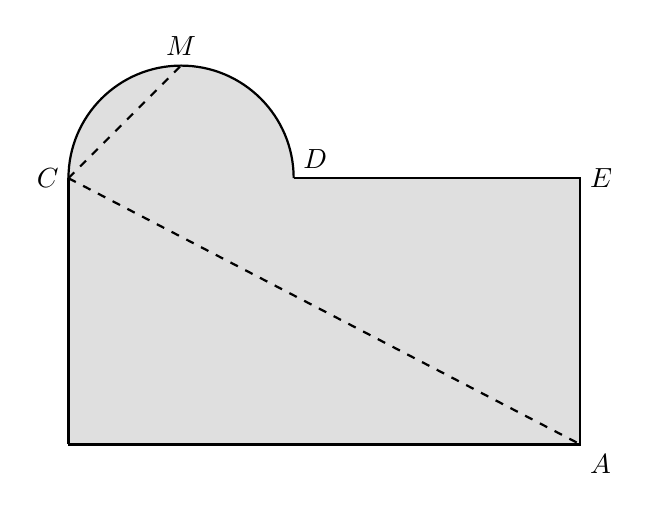
\begin{tikzpicture}[>=stealth, scale=1.3]

    % =================================================================
    % 1. ĐỊNH NGHĨA TỌA ĐỘ CÁC ĐIỂM CHÍNH
    % =================================================================
    \coordinate (Origin) at (0,0); % Góc dưới bên trái
    \coordinate (A) at (5.0,0);
    \coordinate (E) at (5.0,2.6);
    \coordinate (D) at (2.2,2.6);
    \coordinate (C) at (0,2.6);
    
    % Tâm đường tròn của phần mái vòm bán nguyệt nối C và D
    % Khoảng cách CD = 2.2 => bán kính R = 1.1, tâm I tại (1.1, 2.6)
    \coordinate (I) at (1.1,2.6);
    \coordinate (M) at (1.1,3.7); % Đỉnh vòm cao nhất

    % =================================================================
    % 2. TÔ MÀU NỀN XÁM CHO TOÀN BỘ KHỐI HÌNH
    % =================================================================
    \fill[gray!25] (Origin) -- (A) -- (E) -- (D) 
                  arc (0:180:1.1) -- cycle;

    % =================================================================
    % 3. VẼ ĐƯỜNG BIÊN BAO QUANH (NÉT LIỀN ĐẬM)
    % =================================================================
    \draw[thick] (Origin) -- (A) -- (E) -- (D);
    \draw[thick] (D) arc (0:180:1.1);
    \draw[thick] (C) -- (Origin);

    % =================================================================
    % 4. VẼ CÁC ĐOẠN THẲNG NÉT ĐỨT BÊN TRONG HÌNH
    % =================================================================
    % Đường chéo nét đứt nối từ C đến A
    \draw[dashed, thick] (C) -- (A);
    
    % Đường nét đứt nối từ C lên đỉnh vòm M (như trong ảnh gốc đầu tiên)
    \draw[dashed, thick] (C) -- (M);

    % =================================================================
    % 5. GÁN NHÃN CÁC ĐỈNH
    % =================================================================
    \node[below right] at (A) {$A$};
    \node[right] at (E) {$E$};
    \node[above right] at (D) {$D$};
    \node[above] at (M) {$M$};
    \node[left] at (C) {$C$};

\end{tikzpicture}
\end{center}}


% --- CÂU 16 ---
\questionShortAnswer{0}{16}{Có hai trường học cùng ở bên phải một con kênh. Người ta đo được khoảng cách từ cổng trường \( A \) và \( B \) của hai trường học đó đến con kênh lần lượt là \( AD = 650 \, m \), \( BC = 900 \, m \) và \( CD = 4000 \, m \). Người ta muốn xây dựng một trạm xe buýt nằm bên bờ kênh cho học sinh hai trường. Để tiết kiệm chi phí, người ta cần chọn vị trí \( M \) của trạm xe buýt đó trên đoạn \( CD \) sao cho tổng khoảng cách từ hai vị trí \( A, B \) đến vị trí \( M \) là nhỏ nhất. Hãy tìm giá trị nhỏ nhất (đơn vị là mét) của tổng khoảng cách đó (kết quả làm tròn đến hàng đơn vị).

\begin{center}
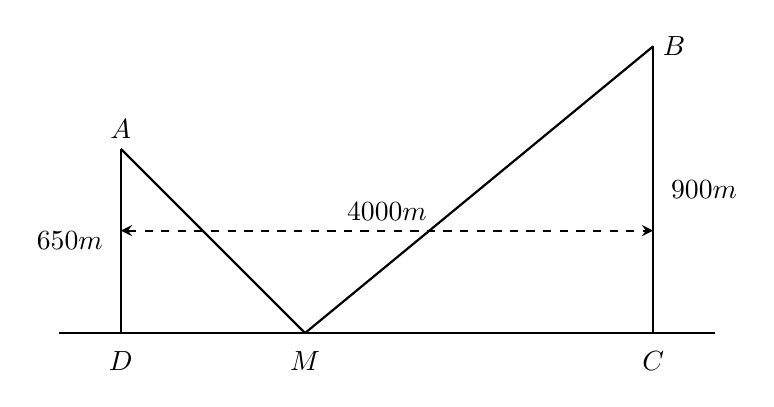
\begin{tikzpicture}[>=stealth, scale=1.3]

    % =================================================================
    % 1. ĐỊNH NGHĨA TỌA ĐỘ CÁC ĐIỂM CHÍNH
    % =================================================================
    \coordinate (D) at (0,0);
    \coordinate (M) at (1.8,0);
    \coordinate (C) at (5.2,0);
    
    % Chiều cao các cột tương ứng tỉ lệ hình vẽ
    \coordinate (A) at (0,1.8);
    \coordinate (B) at (5.2,2.8);

    % Giới hạn trục mặt đất nằm ngang kéo dài hai đầu
    \coordinate (GroundStart) at (-0.6,0);
    \coordinate (GroundEnd) at (5.8,0);

    % Tọa độ cho đường mũi tên nét đứt ở giữa thể hiện khoảng cách ngang
    \coordinate (ArrowLeft) at (0,1.0);
    \coordinate (ArrowRight) at (5.2,1.0);

    % =================================================================
    % 2. VẼ ĐƯỜNG MẶT ĐẤT VÀ CÁC ĐOẠN THẲNG TRÊN HÌNH
    % =================================================================
    % Trục mặt đất nằm ngang
    \draw[thick] (GroundStart) -- (GroundEnd);

    % Hai cột đứng AD và BC
    \draw[thick] (A) -- (D);
    \draw[thick] (B) -- (C);

    % Hai sợi dây căng xiên từ đỉnh xuống điểm M trên mặt đất
    \draw[thick] (A) -- (M);
    \draw[thick] (B) -- (M);

    % =================================================================
    % 3. VẼ ĐƯỜNG MŨI TÊN KÍCH THƯỚC NÉT ĐỨT THỂ HIỆN 4000m
    % =================================================================
    \draw[<->, dashed, thick] (ArrowLeft) -- (ArrowRight);

    % =================================================================
    % 4. GÁN NHÃN CÁC ĐỈNH VÀ THÔNG SỐ SỐ ĐO
    % =================================================================
    % Nhãn các điểm hình học
    \node[above] at (A) {$A$};
    \node[right] at (B) {$B$};
    \node[below=3pt] at (D) {$D$};
    \node[below=3pt] at (M) {$M$};
    \node[below=3pt] at (C) {$C$};

    % Các thông số kích thước, chiều dài
    \node[left=3pt] at (0,0.9) {$650m$};
    \node[right=3pt] at (5.2,1.4) {$900m$};
    \node[above] at (2.6,1.0) {$4000m$};

\end{tikzpicture}
\end{center}}

% --- CÂU 17 ---
\questionShortAnswer{0}{17}{Hai trạm khí tượng đặt tại các vị trí \( A \) và \( B \) cách nhau \( 8 \, \text{km} \). Một trạm thu thập dữ liệu được đặt ở vị trí \( C \) nằm trên đường trung trực của đoạn thẳng \( AB \), cách trung điểm \( M \) của đoạn thẳng \( AB \) một khoảng \( 6 \, \text{km} \). Người ta muốn truyền dữ liệu từ trạm \( C \) đến một vị trí \( I \) nằm giữa đoạn thẳng \( MC \) sau đó chia ra hai nhánh dẫn tới hai nhà máy \( A \) và \( B \) (hình vẽ) thông qua dây dẫn. Tổng độ dài dây dẫn nhỏ nhất bằng bao nhiêu \( km \) (kết quả làm tròn đến hàng phần mười)?

\begin{center}
\begin{tikzpicture}[>=stealth, scale=1.3]

    % =================================================================
    % 1. ĐỊNH NGHĨA TỌA ĐỘ CÁC ĐIỂM CHÍNH
    % =================================================================
    \coordinate (C) at (0,0);
    \coordinate (I) at (2.5,0);
    \coordinate (M) at (4.3,0);
    \coordinate (B) at (4.3,1.7);
    \coordinate (A) at (4.3,-1.7);

    % =================================================================
    % 2. VẼ CÁC ĐOẠN THẲNG TRÊN HÌNH
    % =================================================================
    % Trục nằm ngang đi từ C qua I đến M
    \draw[thick] (C) -- (M);

    % Đoạn thẳng đứng AB đi qua M
    \draw[thick] (A) -- (B);

    % Hai đoạn thẳng xiên nối từ I đến B và A
    \draw[thick] (I) -- (B);
    \draw[thick] (I) -- (A);

    % =================================================================
    % 3. VẼ CÁC ĐIỂM NÚT (CHẤM TRÒN ĐEN)
    % =================================================================
    \fill (C) circle (1.5pt);
    \fill (I) circle (1.5pt);
    \fill (M) circle (1.5pt);
    \fill (B) circle (1.5pt);
    \fill (A) circle (1.5pt);

    % =================================================================
    % 4. GÁN NHÃN CÁC ĐỈNH
    % =================================================================
    \node[below] at (C) {$C$};
    \node[below left] at (I) {$I$};
    \node[right=3pt] at (M) {$M$};
    \node[right=3pt] at (B) {$B$};
    \node[below right] at (A) {$A$};

\end{tikzpicture}
\end{center}}

% --- CÂU 18 ---
\questionShortAnswer{0}{18}{Một đường cáp điện được kéo từ một trạm điện \( A \) ở một bên sông rộng 900 mét đến một nhà máy \( B \) ở bờ bên kia của sông, nhà máy cách trạm điện 3000 mét tính xuôi theo bờ sông. Đường cáp này được mô hình hóa thành đường gấp khúc \( APB \) như hình vẽ, trong đó đoạn \( PB \) đặt trên bờ sông. Giả định rằng tỉ lệ giữa chi phí để kéo 1 mét cáp dưới nước và chi phí kéo 1 mét cáp trên bờ bằng 1,25. Hỏi để tiết kiệm chi phí nhất thì vị trí \( P \) cách nhà máy \( B \) bao nhiêu mét?

\begin{center}
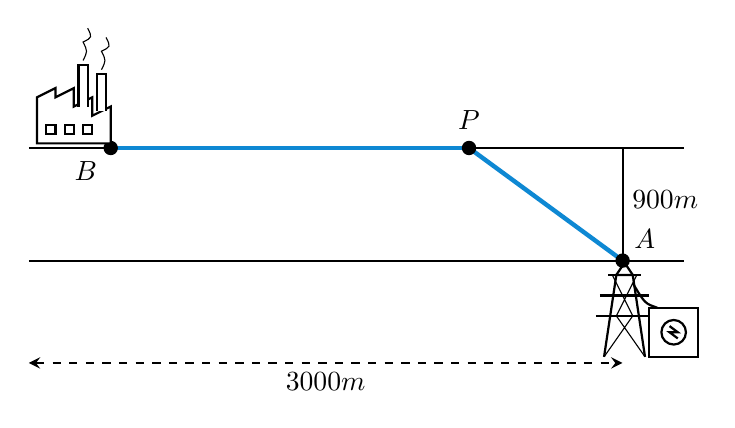
\begin{tikzpicture}[>=stealth, scale=1.3]

    % =================================================================
    % 1. ĐỊNH NGHĨA TỌA ĐỘ CÁC ĐIỂM CHÍNH
    % =================================================================
    \coordinate (B) at (1.0, 1.5);
    \coordinate (P) at (4.5, 1.5);
    \coordinate (A) at (6.0, 0.4);
    
    % Điểm vuông góc từ A lên bờ trên
    \coordinate (H) at (6.0, 1.5);
    
    % Các đường biên bờ sông/đường lộ
    \coordinate (TopStart) at (0.2, 1.5);
    \coordinate (TopEnd) at (6.6, 1.5);
    \coordinate (BottomStart) at (0.2, 0.4);
    \coordinate (BottomEnd) at (6.6, 0.4);

    % =================================================================
    % 2. VẼ HAI ĐƯỜNG BỜ SONG SONG
    % =================================================================
    \draw[thick] (TopStart) -- (TopEnd);
    \draw[thick] (BottomStart) -- (BottomEnd);

    % =================================================================
    % 3. VẼ TUYẾN ĐƯỜNG DÂY ĐIỆN MÀU XANH NỔI BẬT (BP VÀ PA)
    % =================================================================
    \draw[ultra thick, cyan!70!blue] (B) -- (P);
    \draw[ultra thick, cyan!70!blue] (P) -- (A);

    % Đoạn thẳng đứng thể hiện khoảng cách từ A đến bờ đối diện (nét liền mảnh)
    \draw[thick] (H) -- (A);

    % =================================================================
    % 4. VẼ CÁC ĐIỂM NÚT VÀ CÁC BIỂU TƯỢNG MINH HỌA
    % =================================================================
    \fill (B) circle (2pt);
    \fill (P) circle (2pt);
    \fill (A) circle (2pt);

    % --- Nhà máy / Công xưởng tại vị trí B ---
    \begin{scope}[shift={(B)}, scale=0.45, xshift=-0.8cm, yshift=0.1cm]
        \draw[thick, fill=white] (-0.8,0) -- (0.8,0) -- (0.8,0.8) -- (0.4,0.6) -- (0.4,1.0) -- (0,0.8) -- (0,1.2) -- (-0.4,1.0) -- (-0.4,1.2) -- (-0.8,1.0) -- cycle;
        \draw[thick] (-0.6,0.2) rectangle (-0.4,0.4) (-0.2,0.2) rectangle (0,0.4) (0.2,0.2) rectangle (0.4,0.4);
        % Ống khói
        \draw[thick, fill=white] (0.5,0.7) -- (0.5,1.5) -- (0.7,1.5) -- (0.7,0.7);
        \draw[thick, fill=white] (0.1,0.8) -- (0.1,1.7) -- (0.3,1.7) -- (0.3,0.8);
        % Khói bay
        \draw[thin] (0.6,1.6) .. controls (0.7,1.8) .. (0.6,2.0) .. controls (0.8,2.1) .. (0.7,2.3);
        \draw[thin] (0.2,1.8) .. controls (0.3,2.0) .. (0.2,2.2) .. controls (0.4,2.3) .. (0.3,2.5);
    \end{scope}

    % --- Trạm biến áp / Cột điện tại vị trí A ---
    \begin{scope}[shift={(6.1, 0.1)}, scale=0.4, xshift=-0.2cm, yshift=-1.6cm]
        % Khung cột điện hình tháp lưới
        \draw[thick] (-0.5,0) -- (-0.2,2.0) -- (0.2,2.0) -- (0.5,0);
        \draw[thick] (-0.4,2.0) -- (0.4,2.0) (-0.6,1.5) -- (0.6,1.5) (-0.7,1.0) -- (0.7,1.0);
        \draw[thick] (-0.2,2.0) -- (0,2.3) -- (0.2,2.0);
        \draw[thin] (-0.5,0) -- (0.2,1.0) -- (-0.3,2.0) (0.5,0) -- (-0.2,1.0) -- (0.3,2.0);
        % Trạm điện bên cạnh
        \draw[thick, fill=white] (0.6,0) rectangle (1.8,1.2);
        \draw[thick] (1.2,0.6) circle (0.3);
        \draw[thick] (1.1,0.75) -- (1.3,0.6) -- (1.1,0.6) -- (1.3,0.45);
        % Dây điện nối
        \draw[thick] (0.2,1.8) .. controls (0.5,1.3) .. (0.8,1.2);
    \end{scope}

    % =================================================================
    % 5. GÁN NHÃN VÀ KÍ HIỆU CHIỀU DÀI KÍCH THƯỚC
    % =================================================================
    \node[below left=2pt] at (B) {$B$};
    \node[above=3pt] at (P) {$P$};
    \node[above right=1pt] at (A) {$A$};

    % Nhãn khoảng cách 900m
    \node[right] at (6.0, 1.0) {$900m$};

    % Mũi tên nét đứt đôi 3000m phía dưới đáy
    \draw[<->, dashed, thick] (0.2, -0.6) -- (6.0, -0.6);
    \node[below] at (3.1, -0.6) {$3000m$};

\end{tikzpicture}
\end{center}}

% --- CÂU 19 ---
\questionShortAnswer{0}{19}{Một con đường cần được xây dựng giữa hai thành phố \( X \) và \( Y \) nằm ở hai bên đối diện của một con sông có chiều rộng \( 1 \, km \). \( X \) cách sông \( 2 \, km \) và \( Y \) cách sông \( 4 \, km \), khoảng cách giữa hai hình chiếu vuông góc của \( X \) và \( Y \) trên cùng một bên bờ sông là \( 6 \, km \). Một cây cầu sẽ được xây dựng để cho phép giao thông đi qua sông. Vị trí của cây cầu \( CD \) cách \( XX' \) là \( x \, (km) \).

\begin{center}
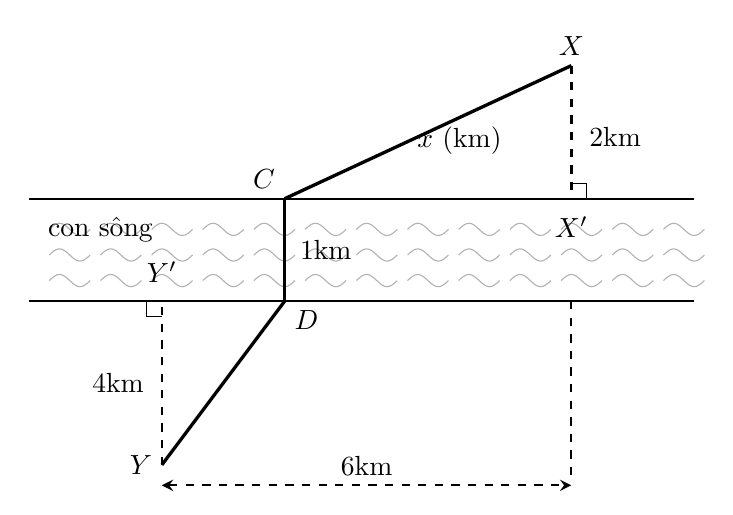
\begin{tikzpicture}[>=stealth, scale=1.3]

    % =================================================================
    % 1. ĐỊNH NGHĨA TỌA ĐỘ CÁC ĐIỂM CHÍNH
    % =================================================================
    % Bờ sông trên cố định tại y = 0.5, bờ dưới cố định tại y = -0.5 (rộng 1km)
    \coordinate (C) at (2.0, 0.5);
    \coordinate (D) at (2.0, -0.5);
    
    \coordinate (X') at (4.8, 0.5);
    \coordinate (X) at (4.8, 1.8);
    
    \coordinate (Y') at (0.8, -0.5);
    \coordinate (Y) at (0.8, -2.1);
    
    % Giới hạn hai bờ sông kéo dài
    \coordinate (TopLeft) at (-0.5, 0.5);
    \coordinate (TopRight) at (6.0, 0.5);
    \coordinate (BottomLeft) at (-0.5, -0.5);
    \coordinate (BottomRight) at (6.0, -0.5);

    % =================================================================
    % 2. VẼ NỀN DÒNG SÔNG (HỌA TIẾT SÓNG NƯỚC)
    % =================================================================
    \foreach \x in {-0.3, 0.2, 0.7, 1.2, 1.7, 2.2, 2.7, 3.2, 3.7, 4.2, 4.7, 5.2, 5.7} {
        \foreach \y in {-0.3, -0.05, 0.2} {
            \draw[shift={(\x,\y)}, xscale=0.5, yscale=0.3, thin, gray!60] 
                (0,0) sin (0.2,0.2) cos (0.4,0) sin (0.6,-0.2) cos (0.8,0);
        }
    }

    % Vẽ hai đường biên song song của con sông
    \draw[thick] (TopLeft) -- (TopRight);
    \draw[thick] (BottomLeft) -- (BottomRight);

    % =================================================================
    % 3. VẼ CÁC TUYẾN ĐƯỜNG LIỀN NÉT VÀ NÉT ĐỨT
    % =================================================================
    % Tuyến đường đi thực tế từ Y -> D -> C -> X
    \draw[very thick] (Y) -- (D);
    \draw[very thick] (D) -- (C);
    \draw[very thick] (C) -- (X);

    % Đường nét đứt thể hiện chiều cao vuông góc
    \draw[dashed, thick] (X) -- (X');
    \draw[dashed, thick] (Y) -- (Y');
    
    % Đường hạ từ X xuống ngang hàng với Y để làm mốc đo khoảng cách 6km
    \draw[dashed, thick] (4.8,-0.5) -- (4.8, -2.2);

    % =================================================================
    % 4. VẼ CÁC KÝ HIỆU GÓC VUÔNG
    % =================================================================
    % Góc vuông tại X'
    \draw[thin] (X') ++(0,0.15) -- ++(0.15,0) -- ++(0,-0.15);
    
    % Góc vuông tại Y'
    \draw[thin] (Y') ++(0,-0.15) -- ++(-0.15,0) -- ++(0,0.15);

    % =================================================================
    % 5. GÁN NHÃN CÁC ĐỈNH VÀ ĐIỀN THÔNG SỐ SỐ ĐO
    % =================================================================
    % Nhãn chữ các điểm nút
    \node[above left] at (C) {$C$};
    \node[below right] at (D) {$D$};
    \node[above] at (X) {$X$};
    \node[below=3pt] at (X') {$X'$};
    \node[above=3pt] at (Y') {$Y'$};
    \node[left] at (Y) {$Y$};

    % Các thông số khoảng cách/chiều dài
    \node[right=2pt] at (2.0, 0.0) {$1\text{km}$};
    \node[right=3pt] at (4.8, 1.1) {$2\text{km}$};
    \node[left=3pt] at (0.8, -1.3) {$4\text{km}$};
    \node[below right] at (3.2, 1.3) {$x\text{ (km)}$};
    \node at (0.2, 0.2) {con sông};

    % Mũi tên nét đứt thể hiện khoảng cách ngang 6km dưới đáy
    \draw[<->, dashed, thick] (0.8, -2.3) -- (4.8, -2.3);
    \node[above] at (2.8, -2.3) {$6\text{km}$};

\end{tikzpicture}
\end{center}

Tìm \( x \) để con đường cần được xây dựng giữa hai thành phố \( X \) và \( Y \) là ngắn nhất.}


% --- CÂU 20 ---
\questionShortAnswer{0}{20}{Cho một bờ hồ hình bán nguyệt có bán kính bằng \( 4 \, km \), đường kính \( PR \) như hình vẽ sau:

\begin{center}
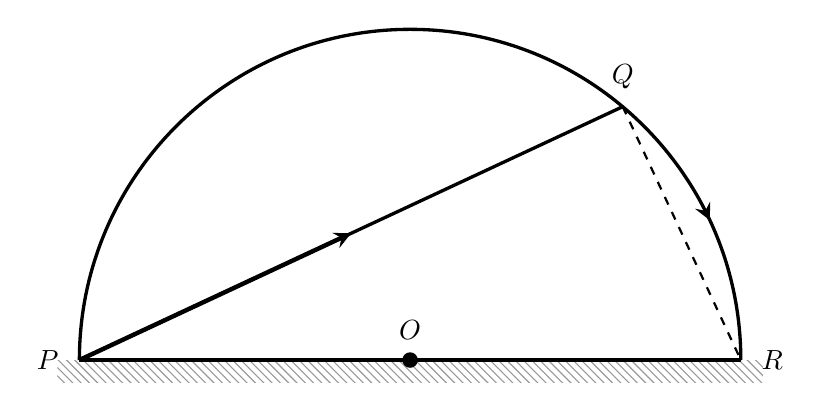
\begin{tikzpicture}[>=stealth, scale=1.4]

    % =================================================================
    % 1. ĐỊNH NGHĨA TỌA ĐỘ VÀ BÁN KÍNH ĐƯỜNG TRÒN
    % =================================================================
    % Tâm đường tròn O đặt tại gốc tọa độ (0,0), bán kính R = 3
    \coordinate (O) at (0,0);
    \coordinate (P) at (-3.0,0);
    \coordinate (R) at (3.0,0);
    
    % Điểm Q nằm trên cung tròn (góc khoảng 50 độ tính từ trục Ox)
    \coordinate (Q) at ({3.0*cos(50)}, {3.0*sin(50)});

    % =================================================================
    % 2. VẼ NỀN GẠCH CHÉO PHÍA DƯỚI ĐƯỜNG KÍNH PR (MẶT ĐẤT)
    % =================================================================
    \fill[pattern=north west lines, pattern color=gray!80] (-3.2,-0.2) rectangle (3.2,0);

    % =================================================================
    % 3. VẼ ĐƯỜNG KÍNH PR VÀ CUNG TRÒN BÁN NGUYỆT
    % =================================================================
    % Đoạn thẳng đường kính PR liền nét, dày dặn
    \draw[very thick] (P) -- (R);

    % Cung tròn nửa trên từ điểm R quay ngược chiều kim đồng hồ đến P
    \draw[very thick] (3.0,0) arc (0:180:3.0);

    % =================================================================
    % 4. VẼ CÁC ĐOẠN THẲNG HÌNH HỌC VÀ MŨI TÊN CHỈ HƯỚNG
    % =================================================================
    % Đoạn thẳng PQ liền nét
    \draw[very thick] (P) -- (Q);
    
    % Mũi tên chỉ hướng nằm chính giữa đoạn thẳng PQ
    \coordinate (MidPQ) at ($ (P)!0.5!(Q) $);
    \draw[->, ultra thick] (P) -- (MidPQ);

    % Đoạn thẳng QR nét đứt
    \draw[dashed, thick] (Q) -- (R);

    % Mũi tên chỉ hướng nằm trên cung tròn từ Q đến R (ở góc khoảng 25 độ)
    \draw[->, ultra thick] ({3.0*cos(26)}, {3.0*sin(26)}) -- ({3.0*cos(25)}, {3.0*sin(25)});

    % =================================================================
    % 5. VẼ CÁC ĐIỂM NÚT (CHẤM TRÒN ĐEN)
    % =================================================================
    \fill (O) circle (2.0pt);

    % =================================================================
    % 6. GÁN NHÃN CÁC ĐỈNH
    % =================================================================
    \node[left=4pt] at (P) {$P$};
    \node[right=4pt] at (R) {$R$};
    \node[above=4pt] at (O) {$O$};
    \node[above=3pt] at (Q) {$Q$};

\end{tikzpicture}
\end{center}

Từ điểm \( P \) anh Bắp chèo một chiếc thuyền với vận tốc \( 5 \, km/h \) đến điểm \( Q \) trên bờ hồ, rồi chạy bộ dọc theo thành hồ đến vị trí \( R \) với vận tốc \( 8 \, km/h \). Thời gian lớn nhất mà anh Bắp di chuyển từ \( P \) đến \( R \) là bao nhiêu (thời gian tính bằng giờ, kết quả làm tròn đến hàng phần trăm)?}

% --- CÂU 21 ---
\questionShortAnswer{0}{21}{Một người chèo một chiếc thuyền xuất phát từ điểm \( A \) trên bờ một con sông thẳng rộng \( 3,5 \, \text{km} \), và muốn đến điểm \( B \) cách điểm \( C \) \( 7 \, \text{km} \). Người này có thể chèo thuyền qua sông đến điểm \( C \) rồi chạy bộ đến \( B \), hoặc anh ta có thể chèo thuyền thẳng đến \( B \). Hoặc anh ta có thể chèo thuyền qua sông đến điểm \( D \) nào đó giữa \( C \) và \( B \) rồi chạy đến điểm \( B \) (hình minh họa).

\begin{center}
\begin{tikzpicture}[>=stealth, scale=1.3]

    % =================================================================
    % 1. ĐỊNH NGHĨA TỌA ĐỘ CÁC ĐIỂM CHÍNH
    % =================================================================
    \coordinate (A) at (1.5, 0);
    \coordinate (C) at (1.5, 2.2);
    \coordinate (D) at (3.2, 2.2);
    \coordinate (B) at (8.5, 2.2);
    
    % Giới hạn hai bờ sông kéo dài sang hai bên
    \coordinate (TopLeft) at (0.2, 2.2);
    \coordinate (TopRight) at (8.8, 2.2);
    \coordinate (BottomLeft) at (0.2, 0);
    \coordinate (BottomRight) at (8.8, 0);

    % =================================================================
    % 2. VẼ NỀN DÒNG SÔNG (HỌA TIẾT SÓNG NƯỚC)
    % =================================================================
    \foreach \x in {0.3, 0.8, 1.3, 1.8, 2.3, 2.8, 3.3, 3.8, 4.3, 4.8, 5.3, 5.8, 6.3, 6.8, 7.3, 7.8, 8.3} {
        \foreach \y in {0.2, 0.5, 0.8, 1.1, 1.4, 1.7, 2.0} {
            \draw[shift={(\x,\y)}, xscale=0.5, yscale=0.3, thin, gray!60] 
                (0,0) sin (0.2,0.2) cos (0.4,0) sin (0.6,-0.2) cos (0.8,0);
        }
    }

    % Vẽ hai đường biên song song của bờ sông
    \draw[thick] (TopLeft) -- (TopRight);
    \draw[thick] (BottomLeft) -- (BottomRight);

    % =================================================================
    % 3. VẼ CÁC VECTOR DI CHUYỂN QUA SÔNG
    % =================================================================
    \draw[->, very thick] (A) -- (C);
    \draw[->, very thick] (A) -- (D);
    \draw[->, very thick] (A) -- (B);

    % =================================================================
    % 4. VẼ BIỂU TƯỢNG NGƯỜI CHÈO THUYỀN TẠI VỊ TRÍ A
    % =================================================================
    \begin{scope}[shift={(A)}, scale=0.45, xshift=-1.8cm, yshift=0.2cm]
        % Sóng nước nhỏ dưới thuyền
        \draw[thin] (-0.2,-0.2) sin (0.2,-0.3) cos (0.6,-0.2) sin (1.0,-0.3);
        % Thân thuyền
        \draw[thick, fill=white] (0,0.2) -- (2.0,0.2) -- (1.7,-0.2) -- (0.3,-0.2) -- cycle;
        \draw[thick] (0,0.2) -- (2.0,0.2);
        % Người chèo thuyền
         \draw[thick] (1,0.8) circle (5pt); % Đầu
        \draw[thick] (1.0,0.65) -- (1.0,0.2); % Thân
        \draw[thick] (1.0,0.5) -- (0.6,0.3) -- (0.8,0.0); % Tay giữ mái chèo
        \draw[thick] (1.0,0.5) -- (1.3,0.3); 
        % Mái chèo
        \draw[thick] (0.4,-0.1) -- (1.4,0.7);
    \end{scope}

    % =================================================================
    % 5. GÁN NHÃN CÁC ĐỈNH VÀ CHÚ THÍCH CHỮ
    % =================================================================
    \node[below=4pt] at (A) {$A$};
    \node[above=4pt] at (C) {$C$};
    \node[above=4pt] at (D) {$D$};
    \node[above=4pt] at (B) {$B$};

    % Độ dài khoảng cách chiều rộng sông
    \node[left=3pt] at (1.5, 1.4) {$3,5km$};

    % Chú thích địa hình "bờ sông" ở trên và dưới
    \node[above] at (5.0, 2.2) {bờ sông};
    \node[below] at (5.0, 0) {bờ sông};

\end{tikzpicture}
\end{center}

Biết rằng vận tốc chèo thuyền của anh ta là \( 5 \, \text{km/h} \) (đã tính vận tốc nước), vận tốc chạy bộ của anh ta là \( 9 \, \text{km/h} \). Trong tất cả các phương án đến \( B \) bằng cách chèo thuyền hoặc chèo thuyền rồi chạy bộ, phương án nhanh nhất có tổng thời gian là bao nhiêu giờ (kết quả làm tròn đến hàng phần trăm)?}

% --- CÂU 22 ---
\questionShortAnswer{0}{22}{Hai nhà máy sản xuất đặt tại các vị trí \( A \) và \( B \) cách nhau \( 4 \, \text{km} \). Một nhà máy cung cấp nước được đặt ở vị trí \( C \) nằm trên đường trung trực của đoạn thẳng \( AB \), cách trung điểm \( M \) của đoạn thẳng \( AB \) một khoảng \( 4 \, \text{km} \). Người ta muốn làm một đường ống dẫn nước từ nhà máy nước \( C \) đến một vị trí \( I \) nằm giữa đoạn thẳng \( MC \) sau đó chia ra hai nhánh dẫn tới hai nhà máy \( A \) và \( B \) (hình vẽ). Hỏi \( I \) cần cách \( C \) bao nhiêu \( \text{km} \) để tổng độ dài đường ống là nhỏ nhất (kết quả làm tròn đến hàng phần trăm)?

\begin{center}
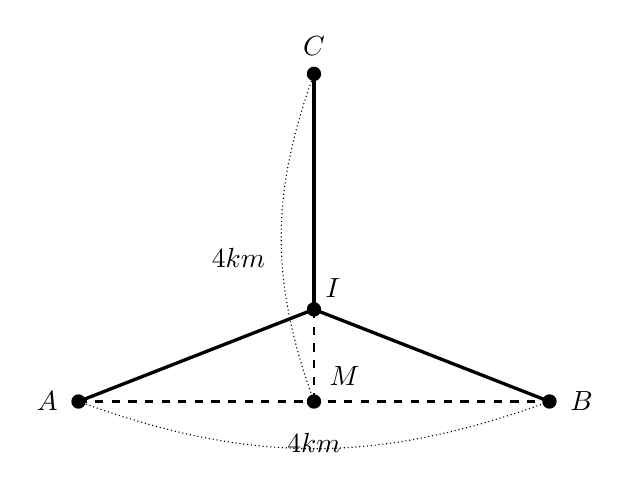
\begin{tikzpicture}[>=stealth, scale=1.3]

    % =================================================================
    % 1. ĐỊNH NGHĨA TỌA ĐỘ CÁC ĐIỂM CHÍNH
    % =================================================================
    \coordinate (M) at (0,0);
    \coordinate (A) at (-2.3,0);
    \coordinate (B) at (2.3,0);
    \coordinate (I) at (0,0.9);
    \coordinate (C) at (0,3.2);

    % =================================================================
    % 2. VẼ CÁC ĐOẠN THẲNG LIỀN NÉT VÀ NÉT ĐỨT
    % =================================================================
    % Đoạn thẳng đứng liền nét IC
    \draw[very thick] (I) -- (C);

    % Hai đoạn xiên liền nét IA và IB
    \draw[very thick] (I) -- (A);
    \draw[very thick] (I) -- (B);

    % Các đoạn thẳng nét đứt thể hiện đường gióng hình học
    \draw[dashed, thick] (A) -- (B);
    \draw[dashed, thick] (M) -- (I);

    % =================================================================
    % 3. VẼ CÁC ĐƯỜNG CONG NÉT CHẤM (MÓC ĐO KÍCH THƯỚC)
    % =================================================================
    % Đường cong biểu diễn khoảng cách 4km từ C xuống M
    \draw[densely dotted, thin] (C) to[out=250, in=110] (M);

    % Đường cong biểu diễn khoảng cách 4km từ A đến B
    \draw[densely dotted, thin] (A) to[out=-20, in=-160] (B);

    % =================================================================
    % 4. VẼ CÁC ĐIỂM NÚT (CHẤM TRÒN ĐEN)
    % =================================================================
    \fill (A) circle (2.0pt);
    \fill (B) circle (2.0pt);
    \fill (M) circle (2.0pt);
    \fill (I) circle (2.0pt);
    \fill (C) circle (2.0pt);

    % =================================================================
    % 5. GÁN NHÃN CÁC ĐỈNH VÀ THÔNG SỐ ĐO KÍCH THƯỚC
    % =================================================================
    \node[above=3pt] at (C) {$C$};
    \node[above right=1pt] at (I) {$I$};
    \node[above right=3pt] at (M) {$M$};
    \node[left=4pt] at (A) {$A$};
    \node[right=4pt] at (B) {$B$};

    % Thông số 4km cho chiều dọc CM
    \node[left=3pt] at (-0.3, 1.4) {$4km$};

    % Thông số 4km cho chiều ngang AB
    \node[below=8pt] at (M) {$4km$};

\end{tikzpicture}
\end{center}}

% --- CÂU 23 ---
\questionShortAnswer{0}{23}{Cho hai vị trí \( A, B \) cách nhau 850 m, cùng nằm về một phía bờ sông như hình vẽ. Khoảng cách từ \( A \) và từ \( B \) đến bờ sông lần lượt là 146 m và 506 m. Một người đi từ \( A \) đến bờ sông để lấy nước mang về \( B \). Đoạn đường ngắn nhất mà người đó có thể đi là bao nhiêu mét (kết quả làm tròn đến hàng đơn vị)?

\begin{center}
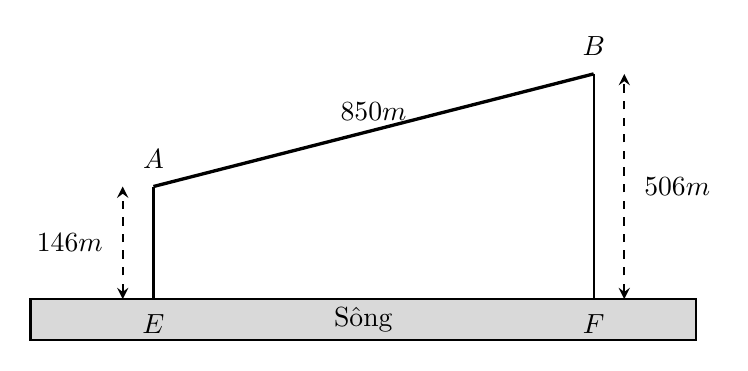
\begin{tikzpicture}[>=stealth, scale=1.3]

    % =================================================================
    % 1. ĐỊNH NGHĨA TỌA ĐỘ CÁC ĐIỂM CHÍNH
    % =================================================================
    % Trục mặt sông nằm ở y = 0
    \coordinate (E) at (1.2, 0);
    \coordinate (F) at (5.5, 0);
    
    % Độ cao các điểm tương ứng với tỉ lệ hình vẽ
    \coordinate (A) at (1.2, 1.1);
    \coordinate (B) at (5.5, 2.2);

    % Giới hạn dải hình chữ nhật của dòng sông
    \coordinate (RiverLeftTop) at (0.0, 0);
    \coordinate (RiverRightBottom) at (6.5, -0.4);

    % =================================================================
    % 2. VẼ DÒNG SÔNG (HÌNH CHỮ NHẬT NỀN XÁM NHẠT)
    % =================================================================
    \draw[thick, fill=gray!30] (RiverLeftTop) rectangle (RiverRightBottom);
    \node at (3.25, -0.2) {Sông};

    % =================================================================
    % 3. VẼ CÁC ĐOẠN THẲNG LỘ TRÌNH VÀ TUYẾN ĐƯỜNG
    % =================================================================
    % Hai đoạn thẳng đứng hạ xuống mặt sông
    \draw[thick] (A) -- (E);
    \draw[thick] (B) -- (F);

    % Đoạn thẳng xiên nối từ A đến B
    \draw[very thick] (A) -- (B);

    % =================================================================
    % 4. VẼ ĐƯỜNG NÉT ĐỨT VÀ MŨI TÊN KÍCH THƯỚC
    % =================================================================
    % Mũi tên nét đứt đôi đo chiều cao bên trái (146m)
    \draw[<->, dashed, thick] (0.9, 0) -- (0.9, 1.1);

    % Mũi tên nét đứt đôi đo chiều cao bên phải (506m)
    \draw[<->, dashed, thick] (5.8, 0) -- (5.8, 2.2);

    % =================================================================
    % 5. GÁN NHÃN CÁC ĐỈNH VÀ THÔNG SỐ SỐ ĐO
    % =================================================================
    % Tên các điểm hình học
    \node[above=3pt] at (A) {$A$};
    \node[above=3pt] at (B) {$B$};
    \node[below=2pt] at (E) {$E$};
    \node[below=2pt] at (F) {$F$};

    % Thông số kích thước chiều dài
    \node[left] at (0.8, 0.55) {$146m$};
    \node[right] at (5.9, 1.1) {$506m$};
    \node[above] at (3.35, 1.65) {$850m$};

\end{tikzpicture}
\end{center}}

% --- CÂU 24 ---
\questionShortAnswer{0}{24}{Trong bài thực hành của môn huấn luyện quân sự có tình huống chiến sĩ phải bơi qua một con sông để tấn công một mục tiêu ở phía bờ bên kia sông. Biết rằng lòng sông rộng \( 500 \, m \) và vận tốc bơi của chiến sĩ bằng một nửa vận tốc chạy trên bộ. Chiến sĩ phải bơi bao nhiêu mét để đến được mục tiêu nhanh nhất, nếu như dòng sông là thẳng, mục tiêu ở cách chiến sĩ \( 1 \, km \) theo đường chim bay?

\begin{center}
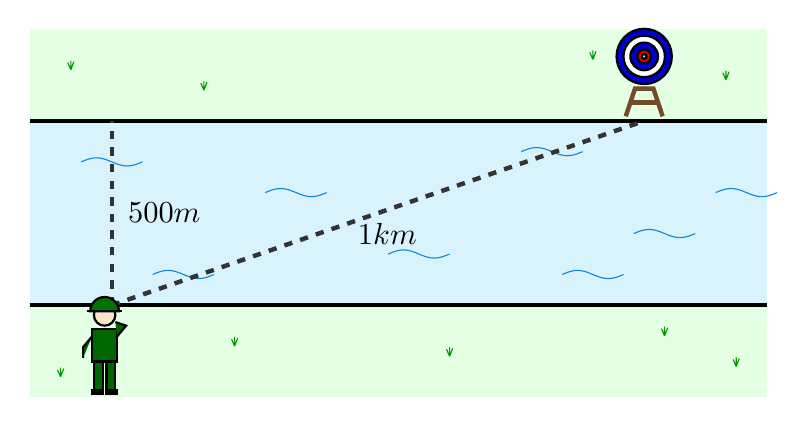
\begin{tikzpicture}[>=stealth, scale=1.3]

    % =================================================================
    % 1. ĐỊNH NGHĨA TỌA ĐỘ CÁC ĐIỂM CHÍNH
    % =================================================================
    % Bờ sông dưới ở y = 0, bờ sông trên ở y = 1.8
    \coordinate (Start) at (0.8, 0);
    \coordinate (Opposite) at (0.8, 1.8);
    \coordinate (Target) at (6.0, 1.8);
    
    % Giới hạn hai bờ sông kéo dài sang hai bên
    \coordinate (TopLeft) at (0, 1.8);
    \coordinate (TopRight) at (7.2, 1.8);
    \coordinate (BottomLeft) at (0, 0);
    \coordinate (BottomRight) at (7.2, 0);

    % =================================================================
    % 2. VẼ NỀN DÒNG SÔNG VÀ HAI BỜ (MÀU XANH NƯỚC BIỂN NHẠT)
    % =================================================================
    % Tô màu xanh cho lòng sông
    \fill[cyan!15] (0,0) rectangle (7.2,1.8);
    
    % Tô màu cỏ xanh nhạt cho hai bờ đất
    \fill[green!10] (0,1.8) rectangle (7.2,2.7);
    \fill[green!10] (0,0) rectangle (7.2,-0.9);

    % Vẽ vài nét gợn sóng nước lăn tăn trên sông
    \foreach \x/\y in {0.5/1.4, 2.3/1.1, 4.8/1.5, 6.7/1.1, 1.2/0.3, 3.5/0.5, 5.2/0.3, 5.9/0.7} {
        \draw[thin, cyan!70!blue] (\x,\y) sin ++(0.15,0.04) cos ++(0.15,-0.04) sin ++(0.15,-0.04) cos ++(0.15,0.04);
    }
    
    % Vẽ vài khóm cỏ nhỏ li ti trên bờ đất
    \foreach \x/\y in {0.4/2.3, 1.7/2.1, 5.5/2.4, 6.8/2.2, 2.0/-0.4, 4.1/-0.5, 6.2/-0.3, 0.3/-0.7, 6.9/-0.6} {
        \draw[thin, green!60!black] (\x,\y) -- ++(0.03,0.08) (\x,\y) -- ++(-0.03,0.07) (\x,\y) -- ++(0,0.09);
    }

    % Vẽ hai đường biên song song của bờ sông (nét liền đen đậm)
    \draw[ultra thick] (TopLeft) -- (TopRight);
    \draw[ultra thick] (BottomLeft) -- (BottomRight);

    % =================================================================
    % 3. VẼ CÁC ĐƯỜNG KÍCH THƯỚC NÉT ĐỨT
    % =================================================================
    % Đường vuông góc thể hiện chiều rộng sông 500m
    \draw[dashed, ultra thick, black!80] (Start) -- (Opposite);
    
    % Đường xiên nối từ vị trí người chiến sĩ đến bia ngắm 1km
    \draw[dashed, ultra thick, black!80] (Start) -- (Target);

    % =================================================================
    % 4. VẼ BIỂU TƯỢNG NGƯỜI LÍNH VÀ BIA TẬP BẮN
    % =================================================================
    % --- Người lính nhỏ tại vị trí bờ dưới ---
    \begin{scope}[shift={(0.8, -0.2)}, scale=0.35, xshift=-0.2cm, yshift=-1.8cm]
        % Chân và quần
        \draw[thick, fill=green!40!black] (-0.3,0) rectangle (-0.05,0.8);
        \draw[thick, fill=green!40!black] (0.05,0) rectangle (0.3,0.8);
        \draw[thick, fill=black] (-0.35,0) rectangle (-0.05,-0.1) (0.05,0) rectangle (0.35,-0.1);
        % Thân áo bọc
        \draw[thick, fill=green!40!black] (-0.35,0.8) rectangle (0.35,1.7);
        % Tay đang gác lên trán suy nghĩ
        \draw[thick, fill=green!40!black] (-0.35,1.5) -- (-0.6,1.2) -- (-0.6,0.9);
        \draw[thick, fill=green!40!black] (0.35,1.5) -- (0.6,1.8) -- (0.3,1.9);
        % Khuôn mặt và mũ cối
        \draw[thick, fill=orange!20] (0,2.1) circle (0.3);
        \draw[thick, fill=green!45!black] (-0.4,2.2) coordinate (H1) arc (180:0:0.4) -- cycle;
        \draw[thick] (-0.48,2.2) -- (0.48,2.2); % Vành mũ
        % Dấu hỏi chấm nhỏ thể hiện sự suy ngẫm gần đầu
        %\node[scale=0.9, right] at (0.4, 2.3) {$\mathbf{?}$};
    \end{scope}

    % --- Bia tập bắn mục tiêu tại bờ trên ---
    \begin{scope}[shift={(Target)}, scale=0.45, yshift=0.1cm]
        % Giá đỡ chân gỗ
        \draw[ultra thick, brown!60!black] (-0.4,0) -- (-0.2,0.6) -- (0.2,0.6) -- (0.4,0);
        \draw[ultra thick, brown!60!black] (-0.3,0.3) -- (0.3,0.3);
        % Bia tâm vòng tròn đồng tâm
        \draw[thick, fill=blue!80!black] (0,1.3) circle (0.6);
        \draw[thick, fill=white] (0,1.3) circle (0.45);
        \draw[thick, fill=blue!80!black] (0,1.3) circle (0.3);
        \draw[thick, fill=red!80!black] (0,1.3) circle (0.15);
        \draw[thick, fill=white] (0,1.3) circle (0.05);
    \end{scope}

    % =================================================================
    % 5. GÁN NHÃN CÁC THÔNG SỐ SỐ ĐO TRÊN HÌNH
    % =================================================================
    % Khoảng cách chiều rộng sông 500m
    \node[right=2pt, scale=1.1] at (0.8, 0.9) {$500m$};

    % Khoảng cách đường xiên dài 1km
    \node[below right, scale=1.1] at (3.1, 0.9) {$1km$};

\end{tikzpicture}
\end{center}}

% --- CÂU 25 ---
\questionShortAnswer{0}{25}{Một con cá hồi bơi ngược dòng nước để vượt một khoảng cách là \( 250 \, \text{km} \). Vận tốc dòng nước là \( 5 \, (\text{km/h}) \). Nếu vận tốc bơi của cá khi nước đứng yên là \( v \, (\text{km/h}) \) thì năng lượng tiêu hao của cá trong \( t \) giờ được cho bởi công thức \( E(v) = cv^3 t \) (trong đó \( c \) là hằng số dương, \( E \) được tính bằng đơn vị Jun). Cá bơi ngược dòng quãng đường \( 250 \, \text{km} \) trong khoảng thời gian \( t \) với vận tốc bằng bao nhiêu \( \text{km/h} \) để năng lượng tiêu hao là thấp nhất?}

% --- CÂU 26 ---
\questionShortAnswer{0}{26}{Có hai xã cùng ở một bên bờ sông. Người ta đo được khoảng cách từ trung tâm \( A, B \) của hai xã đó đến bờ sông lần lượt là \( AA' = 500 \, m; \, BB' = 600 \, m; \, A'B' = 2200 \, m \) (Hình vẽ). Các kĩ sư muốn xây một trạm cung cấp nước sạch nằm bên bờ sông cho người dân hai xã. Để tiết kiệm chi phí, các kĩ sư cần phải chọn vị trí \( M \) của trạm cung cấp nước sạch đó trên đoạn \( A'B' \) sao cho tổng khoảng cách từ hai vị trí \( A, B \) đến vị trí \( M \) là nhỏ nhất. Hỏi tổng khoảng cách đó có giá trị nhỏ nhất là bao nhiêu mét (làm tròn đến hàng đơn vị)?

\begin{center}
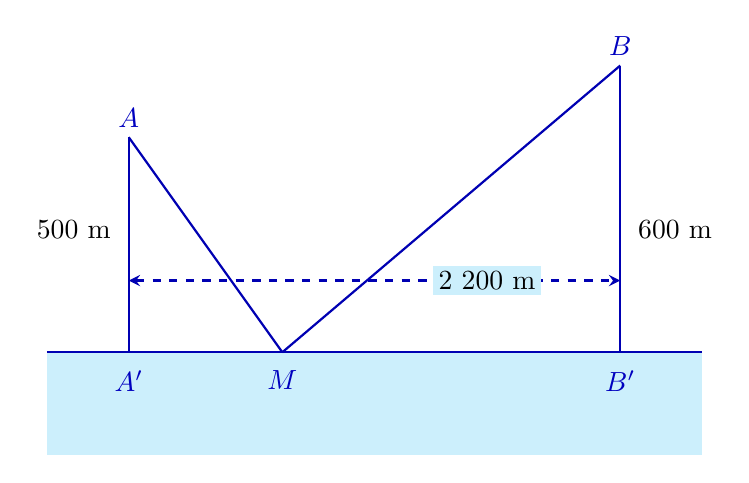
\begin{tikzpicture}[>=stealth, scale=1.3]

    % =================================================================
    % 1. ĐỊNH NGHĨA TỌA ĐỘ CÁC ĐIỂM CHÍNH
    % =================================================================
    \coordinate (A') at (0,0);
    \coordinate (M) at (1.5,0);
    \coordinate (B') at (4.8,0);
    
    % Chiều cao tương ứng tỉ lệ hình vẽ
    \coordinate (A) at (0,2.1);
    \coordinate (B) at (4.8,2.8);

    % Giới hạn trục mặt đất và vùng nước
    \coordinate (GroundStart) at (-0.8,0);
    \coordinate (GroundEnd) at (5.6,0);

    % Tọa độ cho mũi tên nét đứt thể hiện khoảng cách ngang
    \coordinate (ArrowLeft) at (0,0.7);
    \coordinate (ArrowRight) at (4.8,0.7);

    % =================================================================
    % 2. VẼ VÙNG NƯỚC / NỀN PHÍA DƯỚI MẶT ĐẤT
    % =================================================================
    \fill[cyan!20] (-0.8, -1.0) rectangle (5.6, 0);

    % =================================================================
    % 3. VẼ ĐƯỜNG MẶT ĐẤT VÀ CÁC ĐOẠN THẲNG TRÊN HÌNH
    % =================================================================
    % Trục mặt đất nằm ngang màu xanh dương đậm hơn
    \draw[thick, blue!70!black] (GroundStart) -- (GroundEnd);

    % Hai cột đứng AA' và BB'
    \draw[thick, blue!70!black] (A) -- (A');
    \draw[thick, blue!70!black] (B) -- (B');

    % Hai đường xiên từ đỉnh xuống điểm M trên mặt đất
    \draw[thick, blue!70!black] (A) -- (M);
    \draw[thick, blue!70!black] (B) -- (M);

    % =================================================================
    % 4. VẼ ĐƯỜNG MŨI TÊN KÍCH THƯỚC NÉT ĐỨT THỂ HIỆN KHOẢNG CÁCH
    % =================================================================
    \draw[<->, dashed, thick, blue!70!black] (ArrowLeft) -- (ArrowRight);

    % =================================================================
    % 5. GÁN NHÃN CÁC ĐỈNH VÀ THÔNG SỐ SỐ ĐO
    % =================================================================
    % Nhãn các điểm hình học
    \node[above, blue!75!black] at (A) {$A$};
    \node[above, blue!75!black] at (B) {$B$};
    \node[below=3pt, blue!75!black] at (A') {$A'$};
    \node[below=3pt, blue!75!black] at (M) {$M$};
    \node[below=3pt, blue!75!black] at (B') {$B'$};

    % Các thông số kích thước, chiều dài
    \node[left=3pt] at (0,1.2) {$500\text{ m}$};
    \node[right=3pt] at (4.8,1.2) {$600\text{ m}$};
    \node[fill=cyan!20, inner sep=2pt] at (3.5,0.7) {$2\text{ }200\text{ m}$};

\end{tikzpicture}
\end{center}}

\end{document}